
\documentclass[11pt, a4paper, twoside, pdf]{book}
% Opcions 
%  draft : mostra una marca d'aigua
%  bn : no carrega hyperref i la majoria de colors són escala de grisos
\usepackage[bn]{iesbbook}

%%\let\ofrac\frac
%%\let\frac\dfrac
%%\usepackage{pxfonts}

\newcommand{\vso}{\vspace{1cm}}
\newcommand{\vsoo}{\vspace{1.5cm}}
\newcommand{\vsooo}{\vspace{2cm}}
\newcommand{\spen}{{\small \smallpencil}}
\newcommand{\mental}{
\includegraphics[width=0.5cm]{img2/comments}\hspace{0.25cm}}
\newcommand{\ggb}{\includegraphics[width=0.5cm]{img2/geogebra.png}\hspace{0.25cm}}

\makesolucionari
 

\begin{document}
	
\pagestyle{empty}
 \vspace*{0.05cm}


\begin{center}
	
	\shadowoffset{2pt}
	\shadowrgb{0.7,0.7,0.7}
	
	\begin{blueshaded}
		\begin{center} 
			\vspace{0.25cm}
			
			{\fontfamily{phv}\fontsize{38}{57}\selectfont 
				\textbf{\shadowtext{Matemàtiques I}}
				
		
			\vspace{0.25cm}
			{\huge \textbf{1r Batxillerat de ciències}}
			}
				
			\vspace{1cm}
			\shadowoffset{1pt}
			{\Large \textbf{\shadowtext{Sèrie Pràctica}}}
			
			\vspace{0.5cm}
			
			{\Large \normalfont{\textit{3a Edició}}	}	
			\vspace{0.5cm}
		\end{center}
		
	\end{blueshaded}
	
	
	\vspace{1cm}
	
	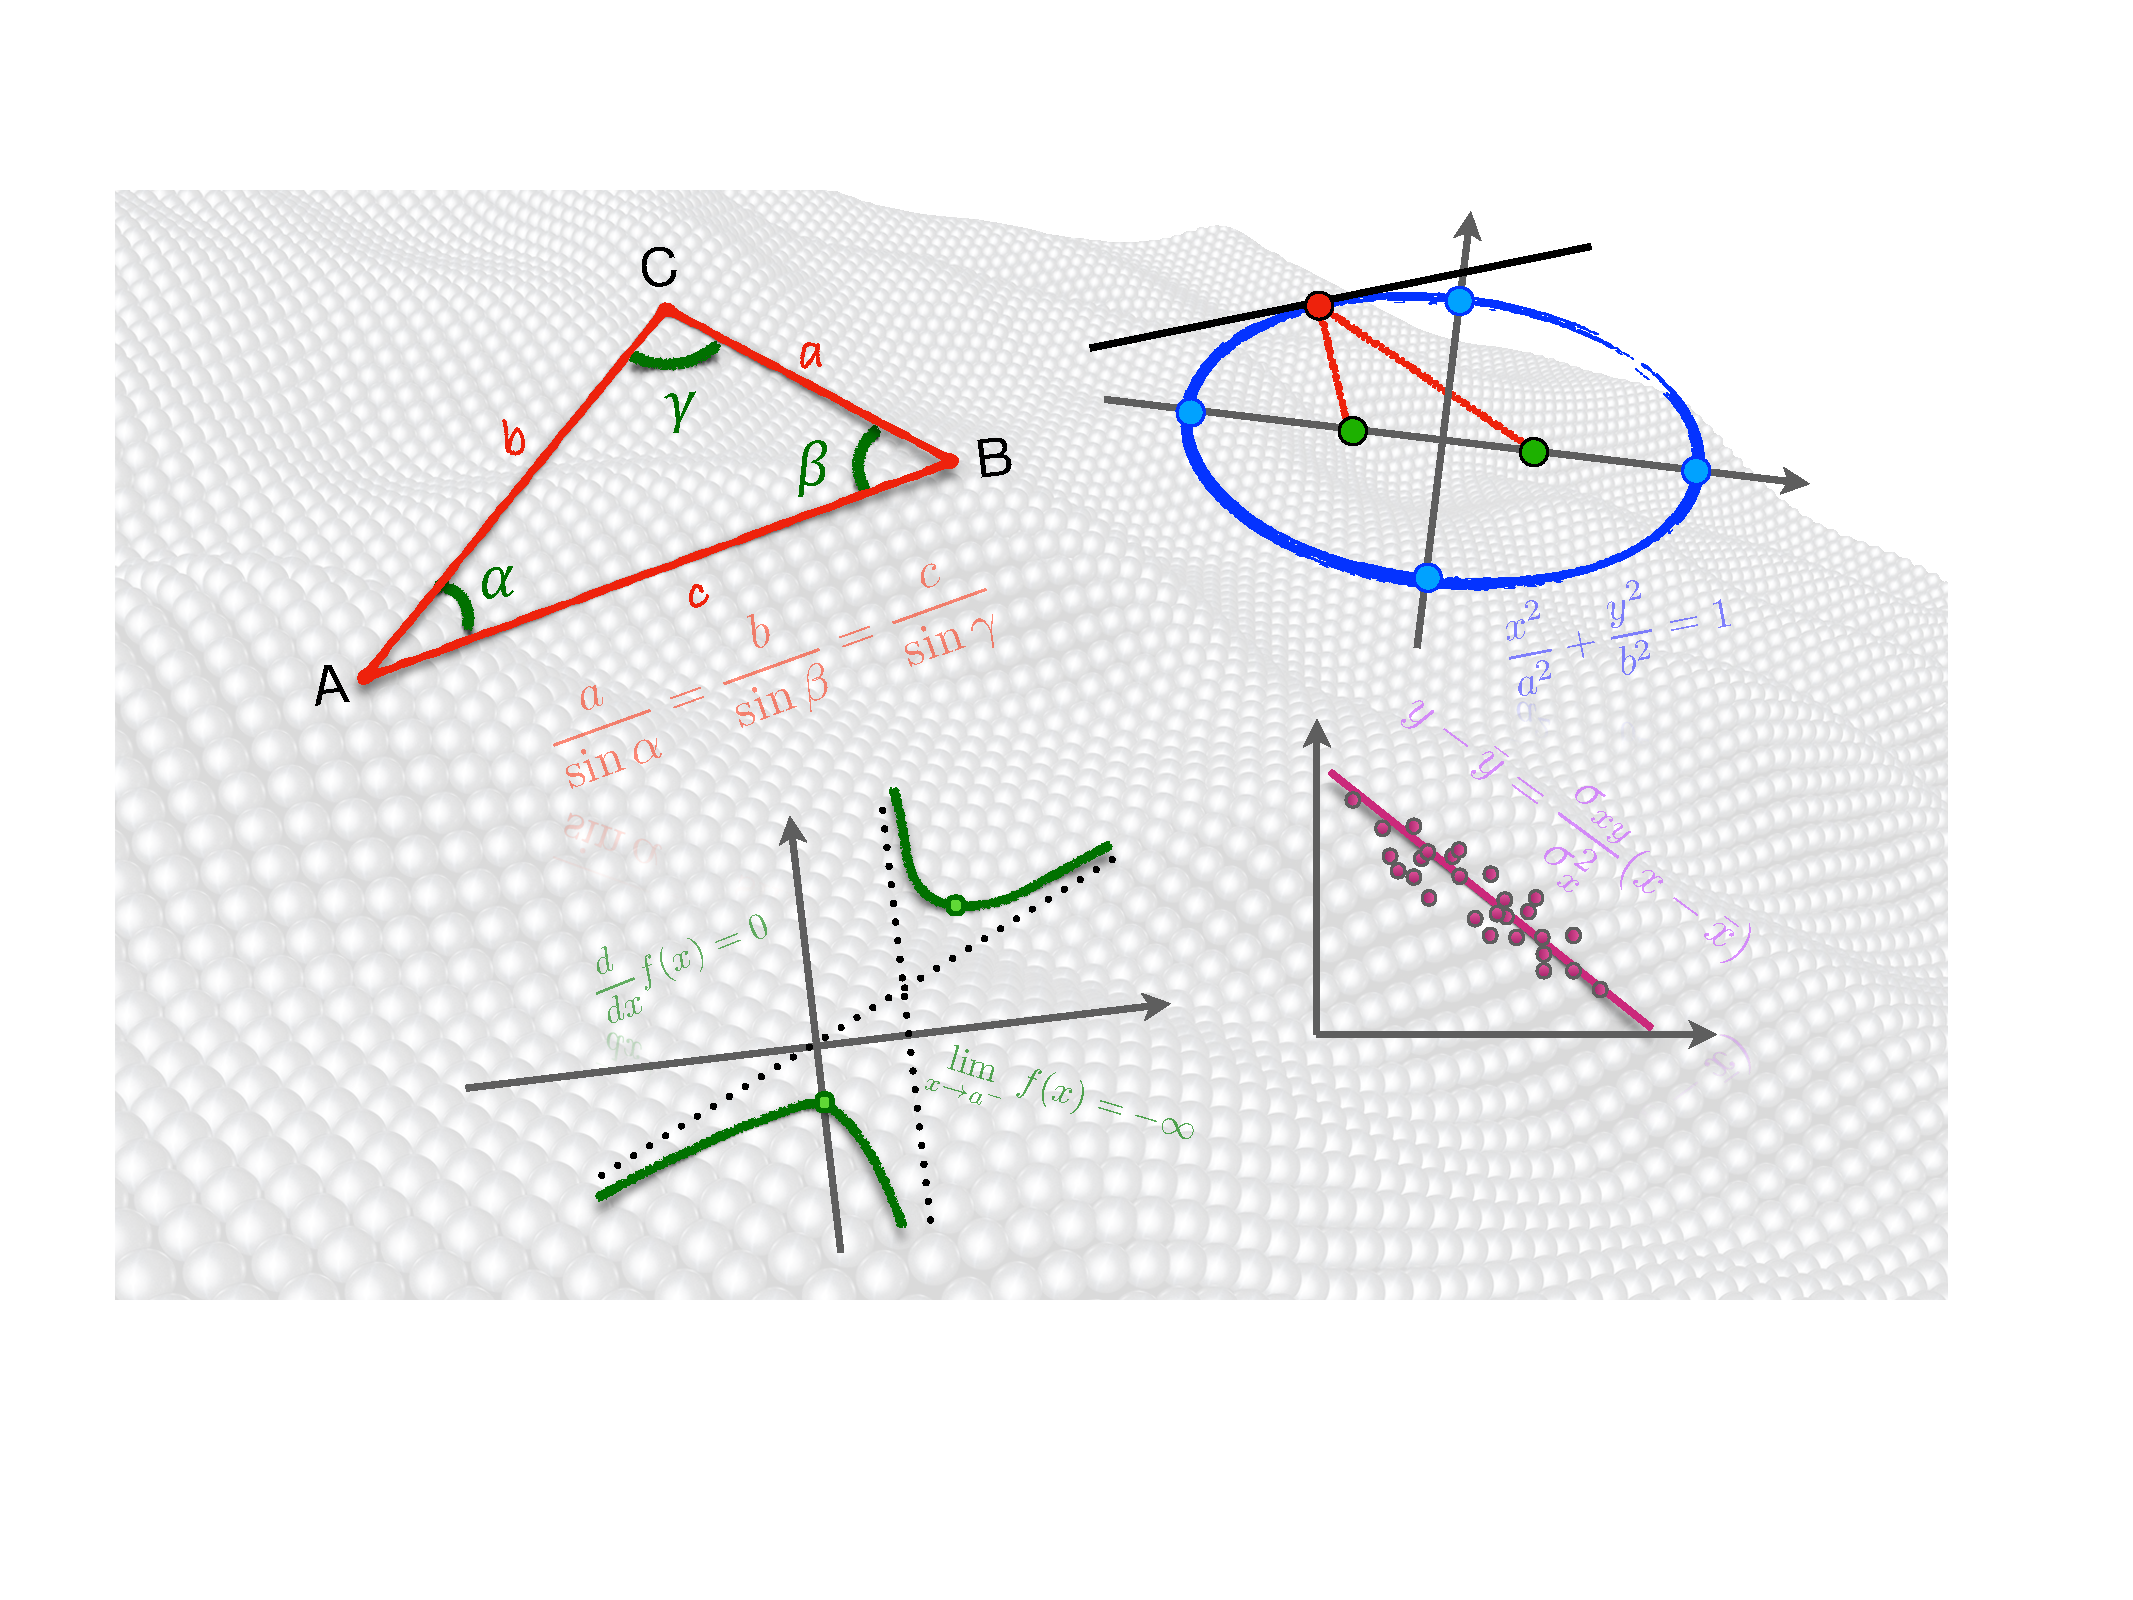
\includegraphics[width=0.9\textwidth]{img-00/portada}
	
	\vspace{1.5cm}
	
	
	\begin{minipage}{0.4\textwidth}
		\begin{center}
			\includegraphics*[width=1.2in]{img-00/ies-binissalem-logo}
			
			\small
			
			\noindent \href{www.iesbinissalem.net}{\textbf{www.iesbinissalem.net}}  
			
		\end{center}
	\end{minipage}
	\begin{minipage}{0.4\textwidth}
		\begin{flushright}
			\textbf{Josep Mulet}
			
			\textit{Departament de Matemàtiques} 
			
			IES Binissalem
		\end{flushright}
	\end{minipage} 
	
	
\end{center}

\newpage

\vspace*{12.9cm}
\begin{center}
	\begin{minipage}{0.5\textwidth}
		Aquesta és una obra derivada de ``\textit{Matematicas 1º de Bachillerato de ciencias. Ejercicios y problemas}'' de Marea Verde de matemàtiques. Per tant, està subjecta a les mateixes condicions de llicència CREATIVE COMMONS que l'obra original.
		
		\noindent \textbf{Edició \LaTeX: \quad \textregistered \,  Josep Mulet Pol}
		
		\noindent \textbf{Versió}: \quad 2018-06-29
		
		\noindent \textbf{Portada}: \quad \textit{Fractal de Julia}.
		
		
		\begin{center}
			\includegraphics*[width=8cm]{img-00/licencia}
		\end{center}
	\end{minipage}
\end{center}

%\clearemptydoublepage
%%\setcounter{page}{1}
%%\fancyfoot[C]{\roman{\thepage}}%


\newpage


\renewcommand{\thepage}{\Roman{page}}% Roman numerals for page counter
\pagestyle{myheadings}
\thispagestyle{empty}
\renewcommand{\headrulewidth}{0pt}
\renewcommand{\footrulewidth}{0pt}

\pagebreak


\dominitoc

\tableofcontents


\newpage

\heading{Currículum LOMCE}

\quad {\footnotesize Extret de \url{http://weib.caib.es/Normativa/Curriculum\_IB/batxillerat\_lomce/matematiques_batx.pdf} }

\begin{center}
	\fontsize{10.1}{13}\selectfont
	\leftmargin=0pt \itemindent=0pt 
	\begin{tabular}{|p{0.5\textwidth}|p{0.5\textwidth}|} \hline
		
		\rowcolor{lightgray} \textbf{BLOC: Nombres i Àlgebra} & \textbf{BLOC: Geometria} \\ \hline
		
		
		\begin{itemize}
			
			\item Nombres reals: necessitat del seu estudi per a la comprensió de la realitat. 
			
			\item Valor absolut. Desigualtats. Distàncies en la recta real. Intervals i entorns. 
			
			\item Aproximació i errors. Notació científica.
			
			\item Nombres complexos. Forma binomial i polar. Representacions gràfiques. Operacions elementals. Fórmula de Moivre.
			
			\item Successions numèriques: terme general, monotonia i acotació. El nombre e.
			
			\item Logaritmes decimals i neperians. Equacions logarítmiques i exponencials.
			
			\item Plantejament i resolució de problemes de la vida quotidiana mitjançant equacions i inequacions. Interpretació gràfica.
			
			\item Resolució d’equacions no algebraiques senzilles.
			Mètode de Gauss per a la resolució i interpretació de sistemes d’equacions lineals.
		\end{itemize}
		
		&
		
		\begin{itemize}
			
			\item 	Mesura d’un angle en radiants.
			
			\item Raons trigonomètriques d’un angle qualsevol. Raons trigonomètriques dels angles suma i diferència d’altres dos, doble i meitat. Fórmules de  transformacions trigonomètriques.
			
			\item Teoremes. Resolució d’equacions trigonomètriques senzilles.
			
			\item Resolució de triangles. Resolució de problemes geomètrics diversos.
			
			\item Vectors lliures en el pla. Operacions geomètriques.
			
			\item Producte escalar. Mòdul d’un vector. Angle de dos vectors.
			
			\item Bases ortogonals i ortonormals.
			
			\item Geometria mètrica plana. Equacions de la recta. Posicions relatives de rectes. Distàncies i angles. Resolució de problemes.
			
			\item Llocs geomètrics en el pla.
			
			\item Còniques. Circumferència, el·lipse, hipèrbola i paràbola. Equació i elements.
			
			
		\end{itemize}
		\\ \hline
		
		\rowcolor{lightgray}  \textbf{BLOC: Anàlisi} & \textbf{BLOC: Estadística i probabilitat}  \\ \hline
		
		\begin{itemize}
			
			\item 	Funcions reals de variable real.
			
			\item Funcions elementals: polinòmiques, racionals senzilles, valor absolut, arrel, trigonomètriques i les seves inverses, exponencials, logarítmiques i funcions definides a trossos.
			
			\item Operacions i composició de funcions. Funció inversa. Funcions d’oferta i demanda.
			
			\item Concepte de límit d’una funció en un punt i en l’infinit. Càlcul de límits. Límits laterals. Indeterminacions.
			
			\item Continuïtat d’una funció. Estudi de discontinuïtats.
			
			\item Derivada d’una funció en un punt. Interpretació geomètrica de la derivada de la funció en un punt. Recta tangent i normal.
			
			\item Funció derivada. Càlcul de funcions derivades. Regla de la cadena.
			
			\item Representació gràfica de funcions.
			
		\end{itemize}		
		&
		
		\begin{itemize}
			\item 	Estadística descriptiva bidimensional:
			Taules de contingència.
			
			\item Distribució conjunta i distribucions marginals.
			
			\item Mitjanes i desviacions típiques marginals.
			
			\item Distribucions condicionades.
			
			\item Independència de variables estadístiques.
			
			\item Estudi de la dependència de dues variables estadístiques. 
			
			\item Representació gràfica: Núvol de punts.
			
			\item Dependència lineal de dues variables estadístiques. 
			
			\item Covariància i correlació: Càlcul i interpretació del coeficient de correlació lineal.
			
			\item Regressió lineal. Estimació. Prediccions estadístiques i fiabilitat de les mateixes.
		\end{itemize}		
		\\ \hline
		
		
	\end{tabular}	
\end{center}

\cleartorightpage
 

\vspace*{2cm} 
\heading{Símbols}

\begin{center}
	\renewcommand{\arraystretch}{1.5}
	\begin{longtable}[h]{>{\raggedleft\arraybackslash}p{0.19\textwidth}|p{0.78\textwidth}}
		{\bfseries Símbol} & {\bfseries Significat} \\ \hline
		
		\simbolclau & Problema clau amb solució al final del llibre.  \\ \hline
		
		\simbolcompass & A més de la solució, proporciona orientacions per arribar a ella.  \\ \hline
		
		\simbolsearch & Problema que requereix d'investigació o recerca d'informació.  \\ \hline
		
		\ggb & Activitat adequada per realitzar amb el programa Geogebra.  \\ \hline
		
		\begin{center}
\includegraphics[width=1cm]{img-00/video-164}\par {\footnotesize Vídeo 132:}\end{center} & Explicació en vídeo dels continguts de l'apartat. El número de vídeo correspon a la numeració emprada en https://piworld.es 
		
		\\ \hline
		\hot[2] & Problema amb un cert grau de dificultat. \\ [0.25cm] \hline
		\spen & Activitat que es pot contestar en el llibre mateix. \\ [0.25cm] \hline 
		\mental & Activitat que es pot resoldre mentalment o en veu alta.
	\end{longtable}
\end{center}
\vspace{1cm} 

\heading{Recursos}

\begin{center}
	\renewcommand{\arraystretch}{1.5}
	\begin{longtable}[h]{>{\raggedleft\arraybackslash}p{0.2\textwidth}|p{0.8\textwidth}}
		\hline
		\textbf{piWorld}
		
		
\includegraphics[height=1.5cm]{img-00/piworld}
		& Plataforma d'aprenentatge. Conté explicacions en vídeo i activitats interactives. Requereix usuari i contrasenya. \newline
		\quad \href{https://piworld.es}{\href{https://piworld.es}{https://piworld.es}}
		\\ \hline
		\textbf{Geogebra} 
		
		\includegraphics[height=1.5cm]{img-00/geogebra}
		& Programa lliure de geometria dinàmica en dues i tres dimensions.
		Ideal pels temes de funcions i geometria.\newline
		\quad  \href{https://www.geogebra.org/download}{\href{https://www.geogebra.org/graphing}{https://www.geogebra.org/graphing}}
		\\ \hline
		\textbf{Calculadora WIRIS}
		
		
		
\includegraphics[height=2cm]{img-00/wiris}
		& Calculadora per al càlcul simbòlic. Nova versió Web \par \quad  \href{https://calcme.com/a}{https://calcme.com/a}
		
		La versió antiga la trobareu a \par \quad  \href{http://www.wiris.net/educa.madrid.org/wiris/es/cas.html}{http://www.wiris.net/educa.madrid.org/wiris/es/cas.html}
		
		Atenció: requereix el plugin de Java i no funciona en dispositius mòbils.
		\\ \hline
		
	\end{longtable}
\end{center}



\pagestyle{fancy}

 
  
\mypart[Fractal de Mandelbrot. La bellesa dels nombres complexos.]{ARITMÈTICA, ÀLGEBRA I TRIGONOMETRIA}{img2/bloc1}

\vspace*{\fill}
\begin{center}
	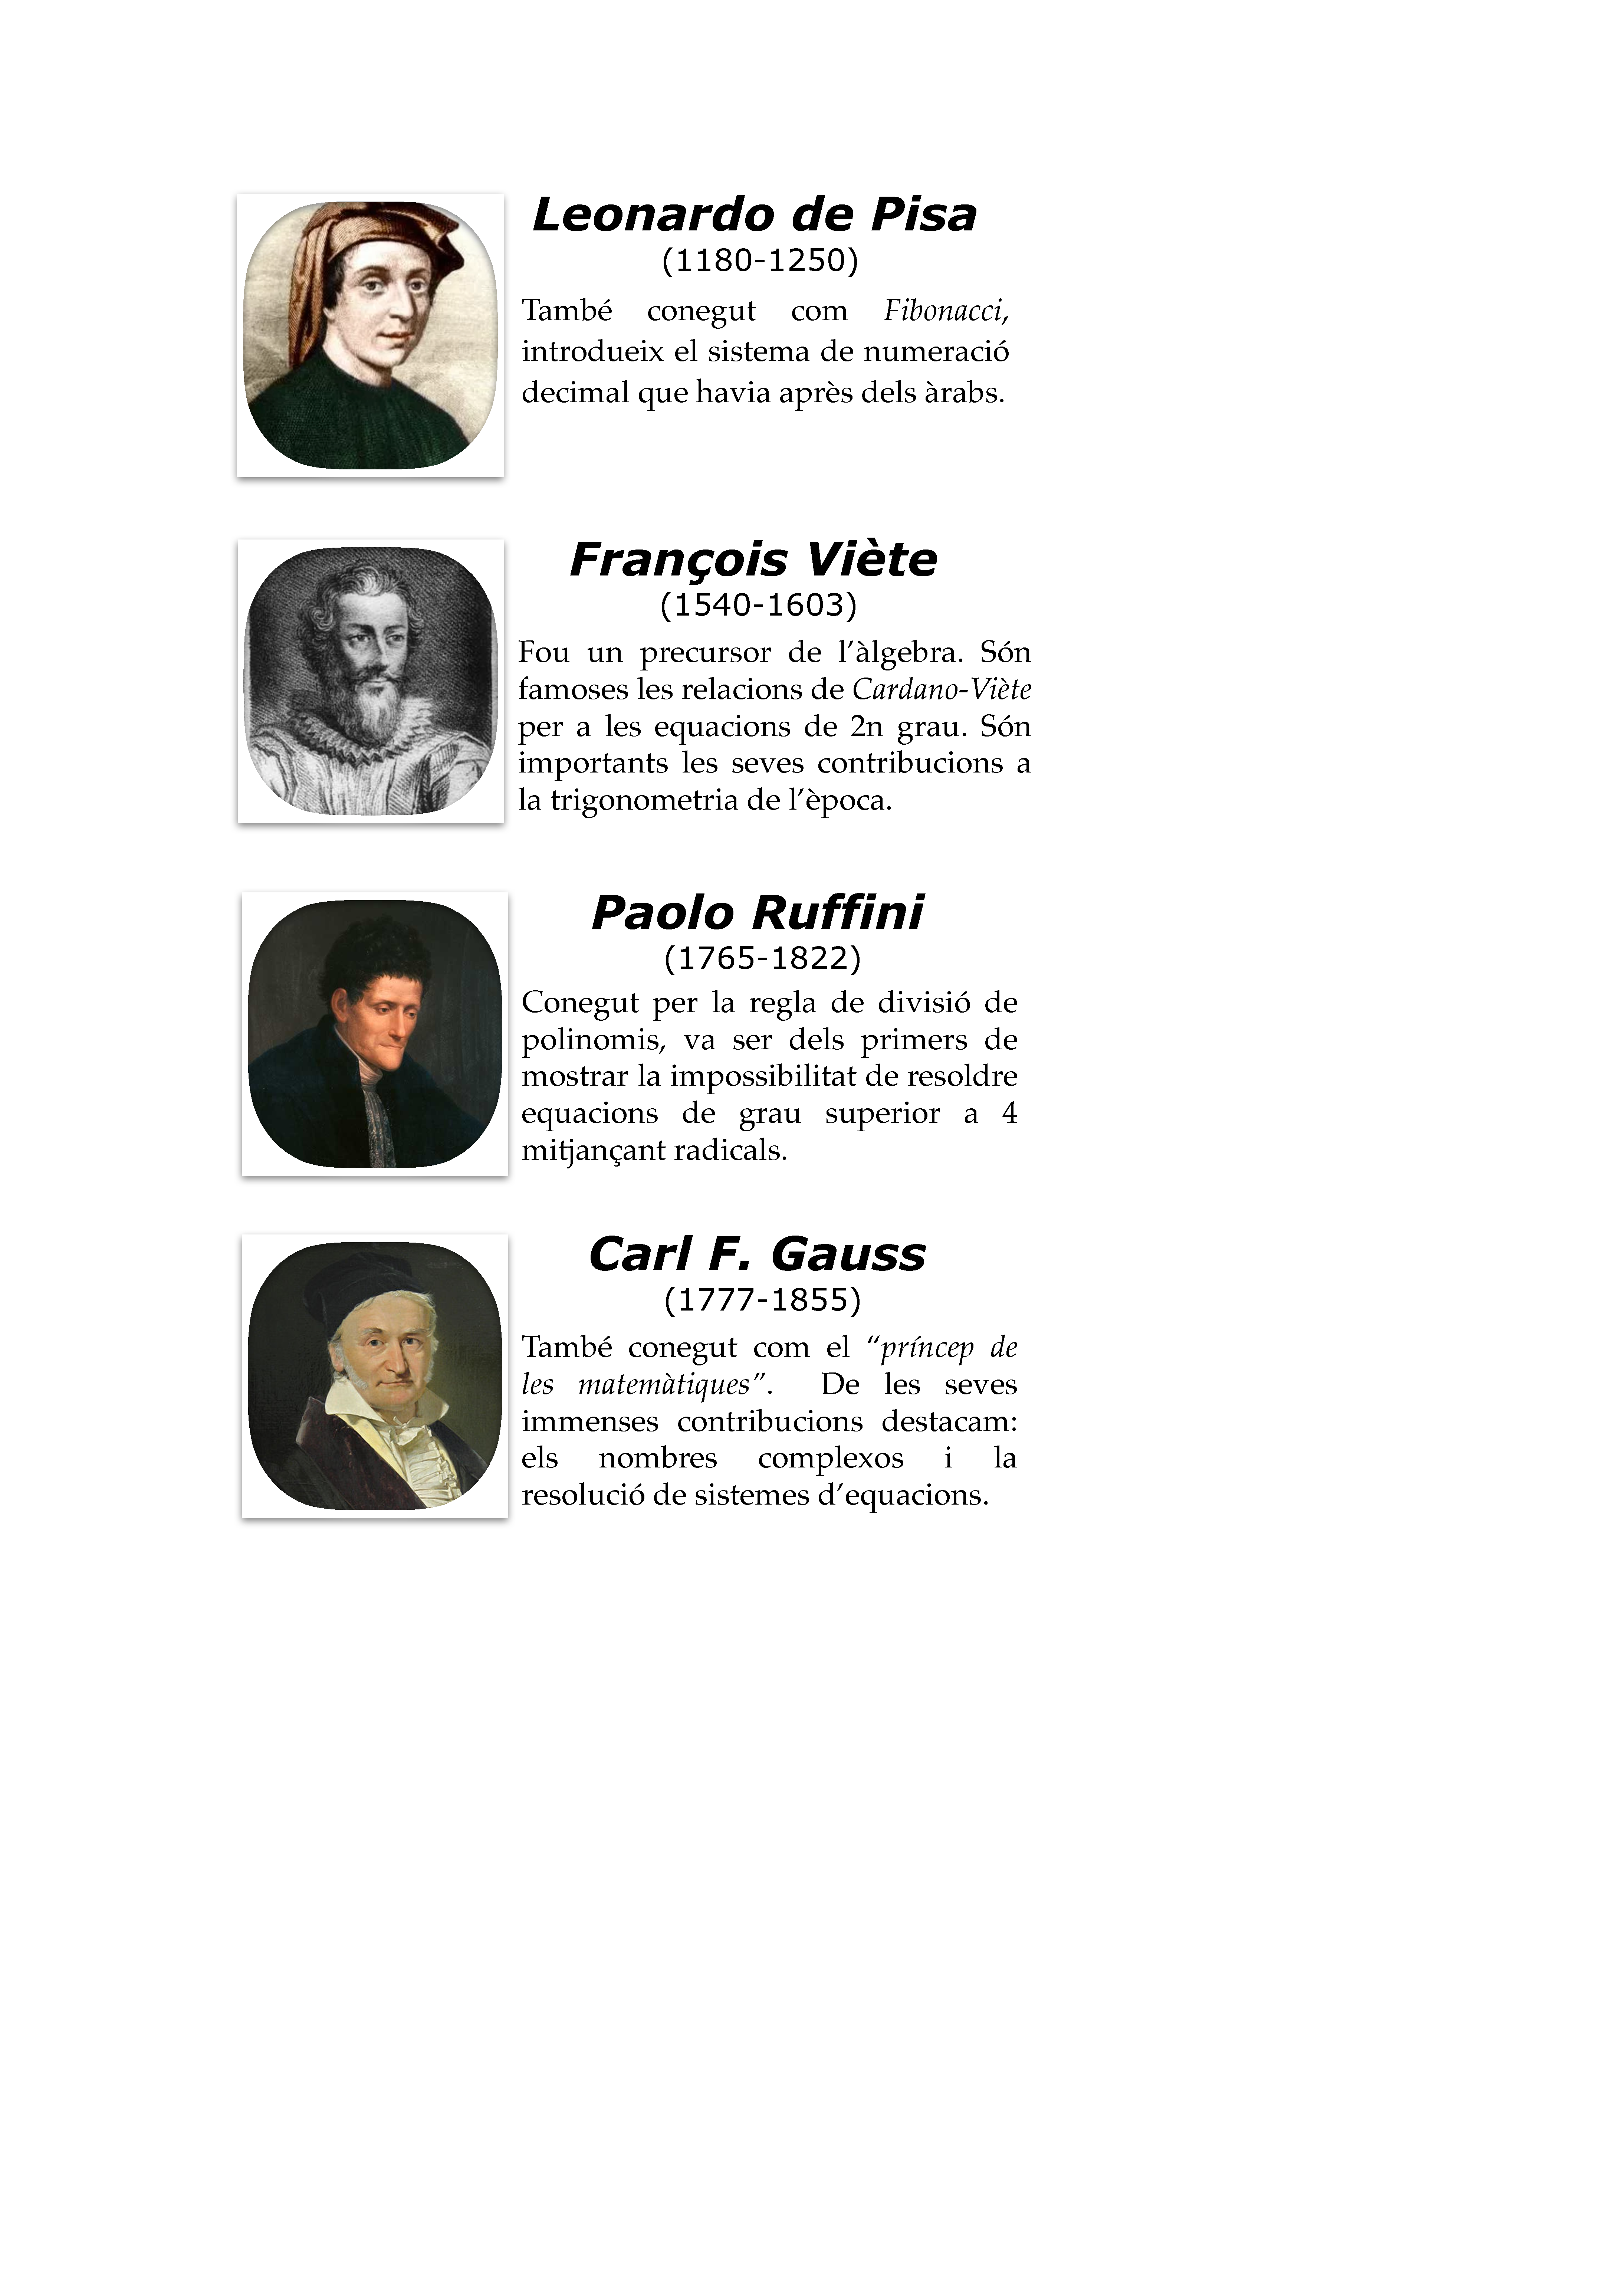
\includegraphics[width=0.65\textwidth]{img2/bloc1-historia}
\end{center}
\vspace*{\fill}

\include{chap-reals}
\include{chap-algebra}
\include{chap-trigonometria}
\include{chap-complexos}
 
%%%%% Activitats de bloc 1
\include{bloc1}

\mypart[L'anàlisi de sèries temporals és cabdal en la vida quotidiana.]{ANÀLISI DE FUNCIONS}{img2/bloc2}
 
\vspace*{\fill}
\begin{center}
	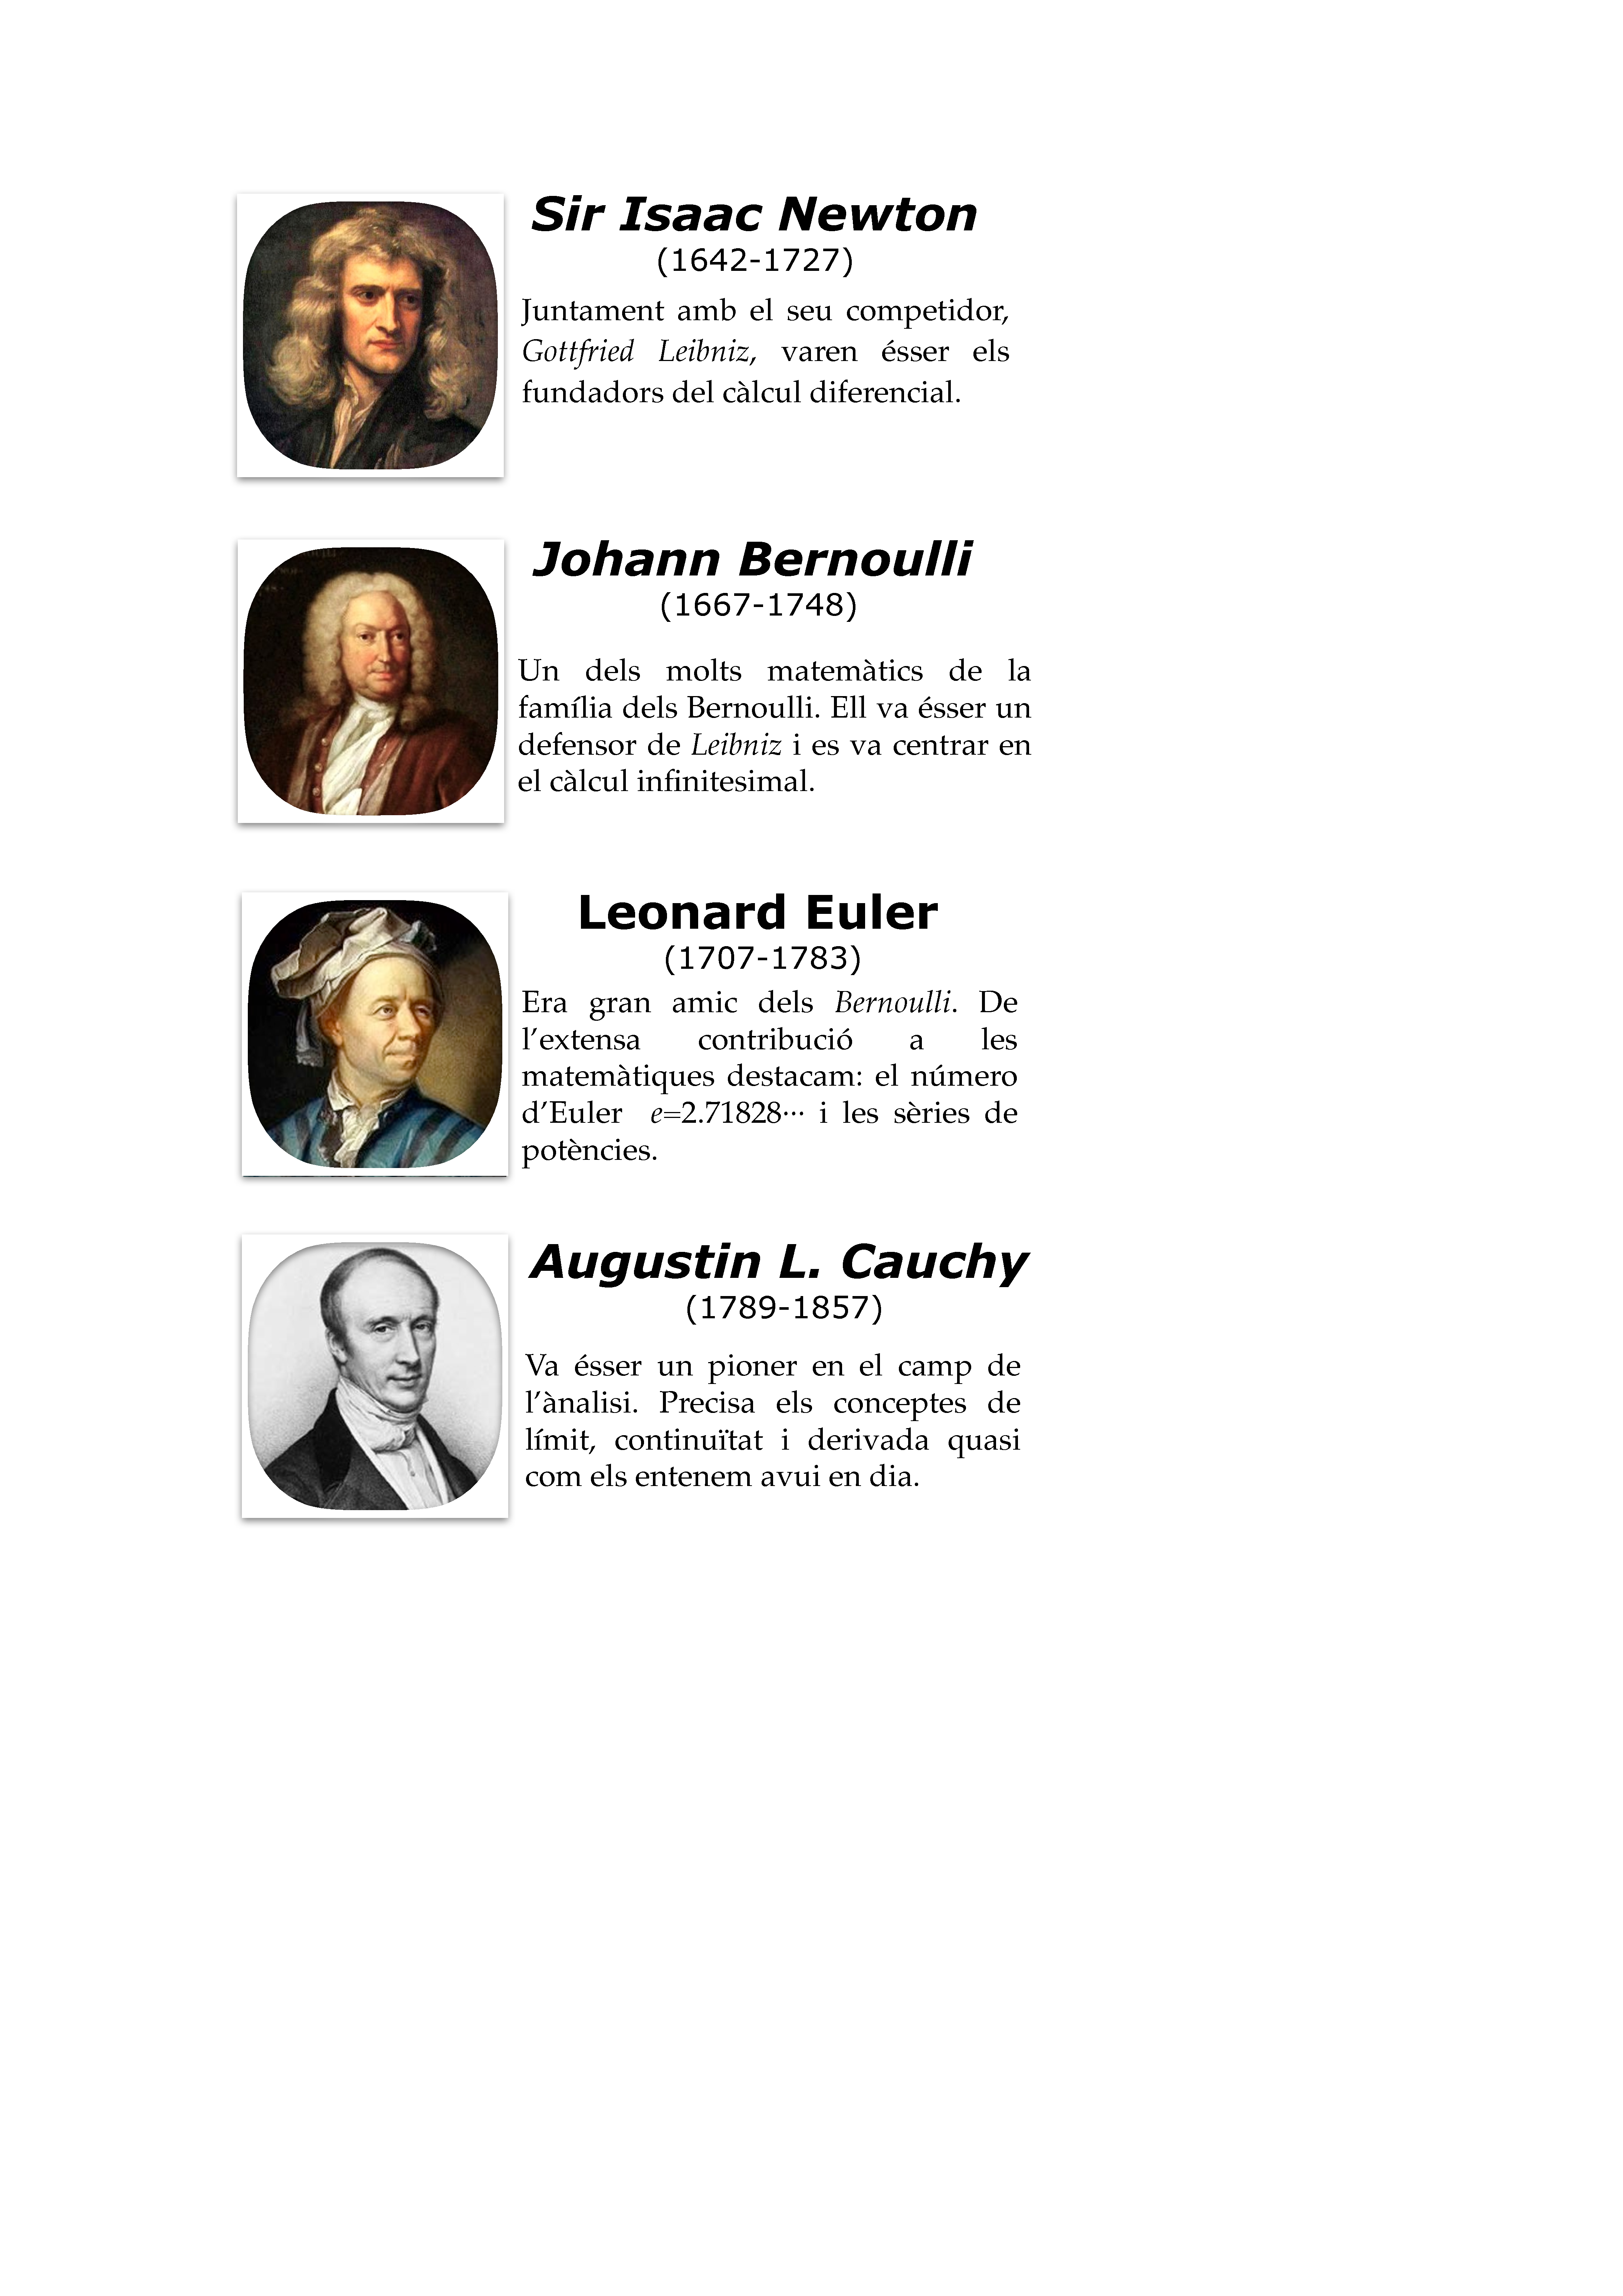
\includegraphics[width=0.65\textwidth]{img2/bloc2-historia}
\end{center}
\vspace*{\fill} 
 
\include{chap-funcelemental}
\include{chap-limits}
\include{chap-derivades}

%%%%% Activitats de bloc 2
\include{bloc2}


  
\mypart[La naturalesa està escrita en llenguatge matemàtic. --Galileo Galilei--]{GEOMETRIA EN EL PLA}{img2/bloc3}

\vspace*{\fill}
\begin{center}
	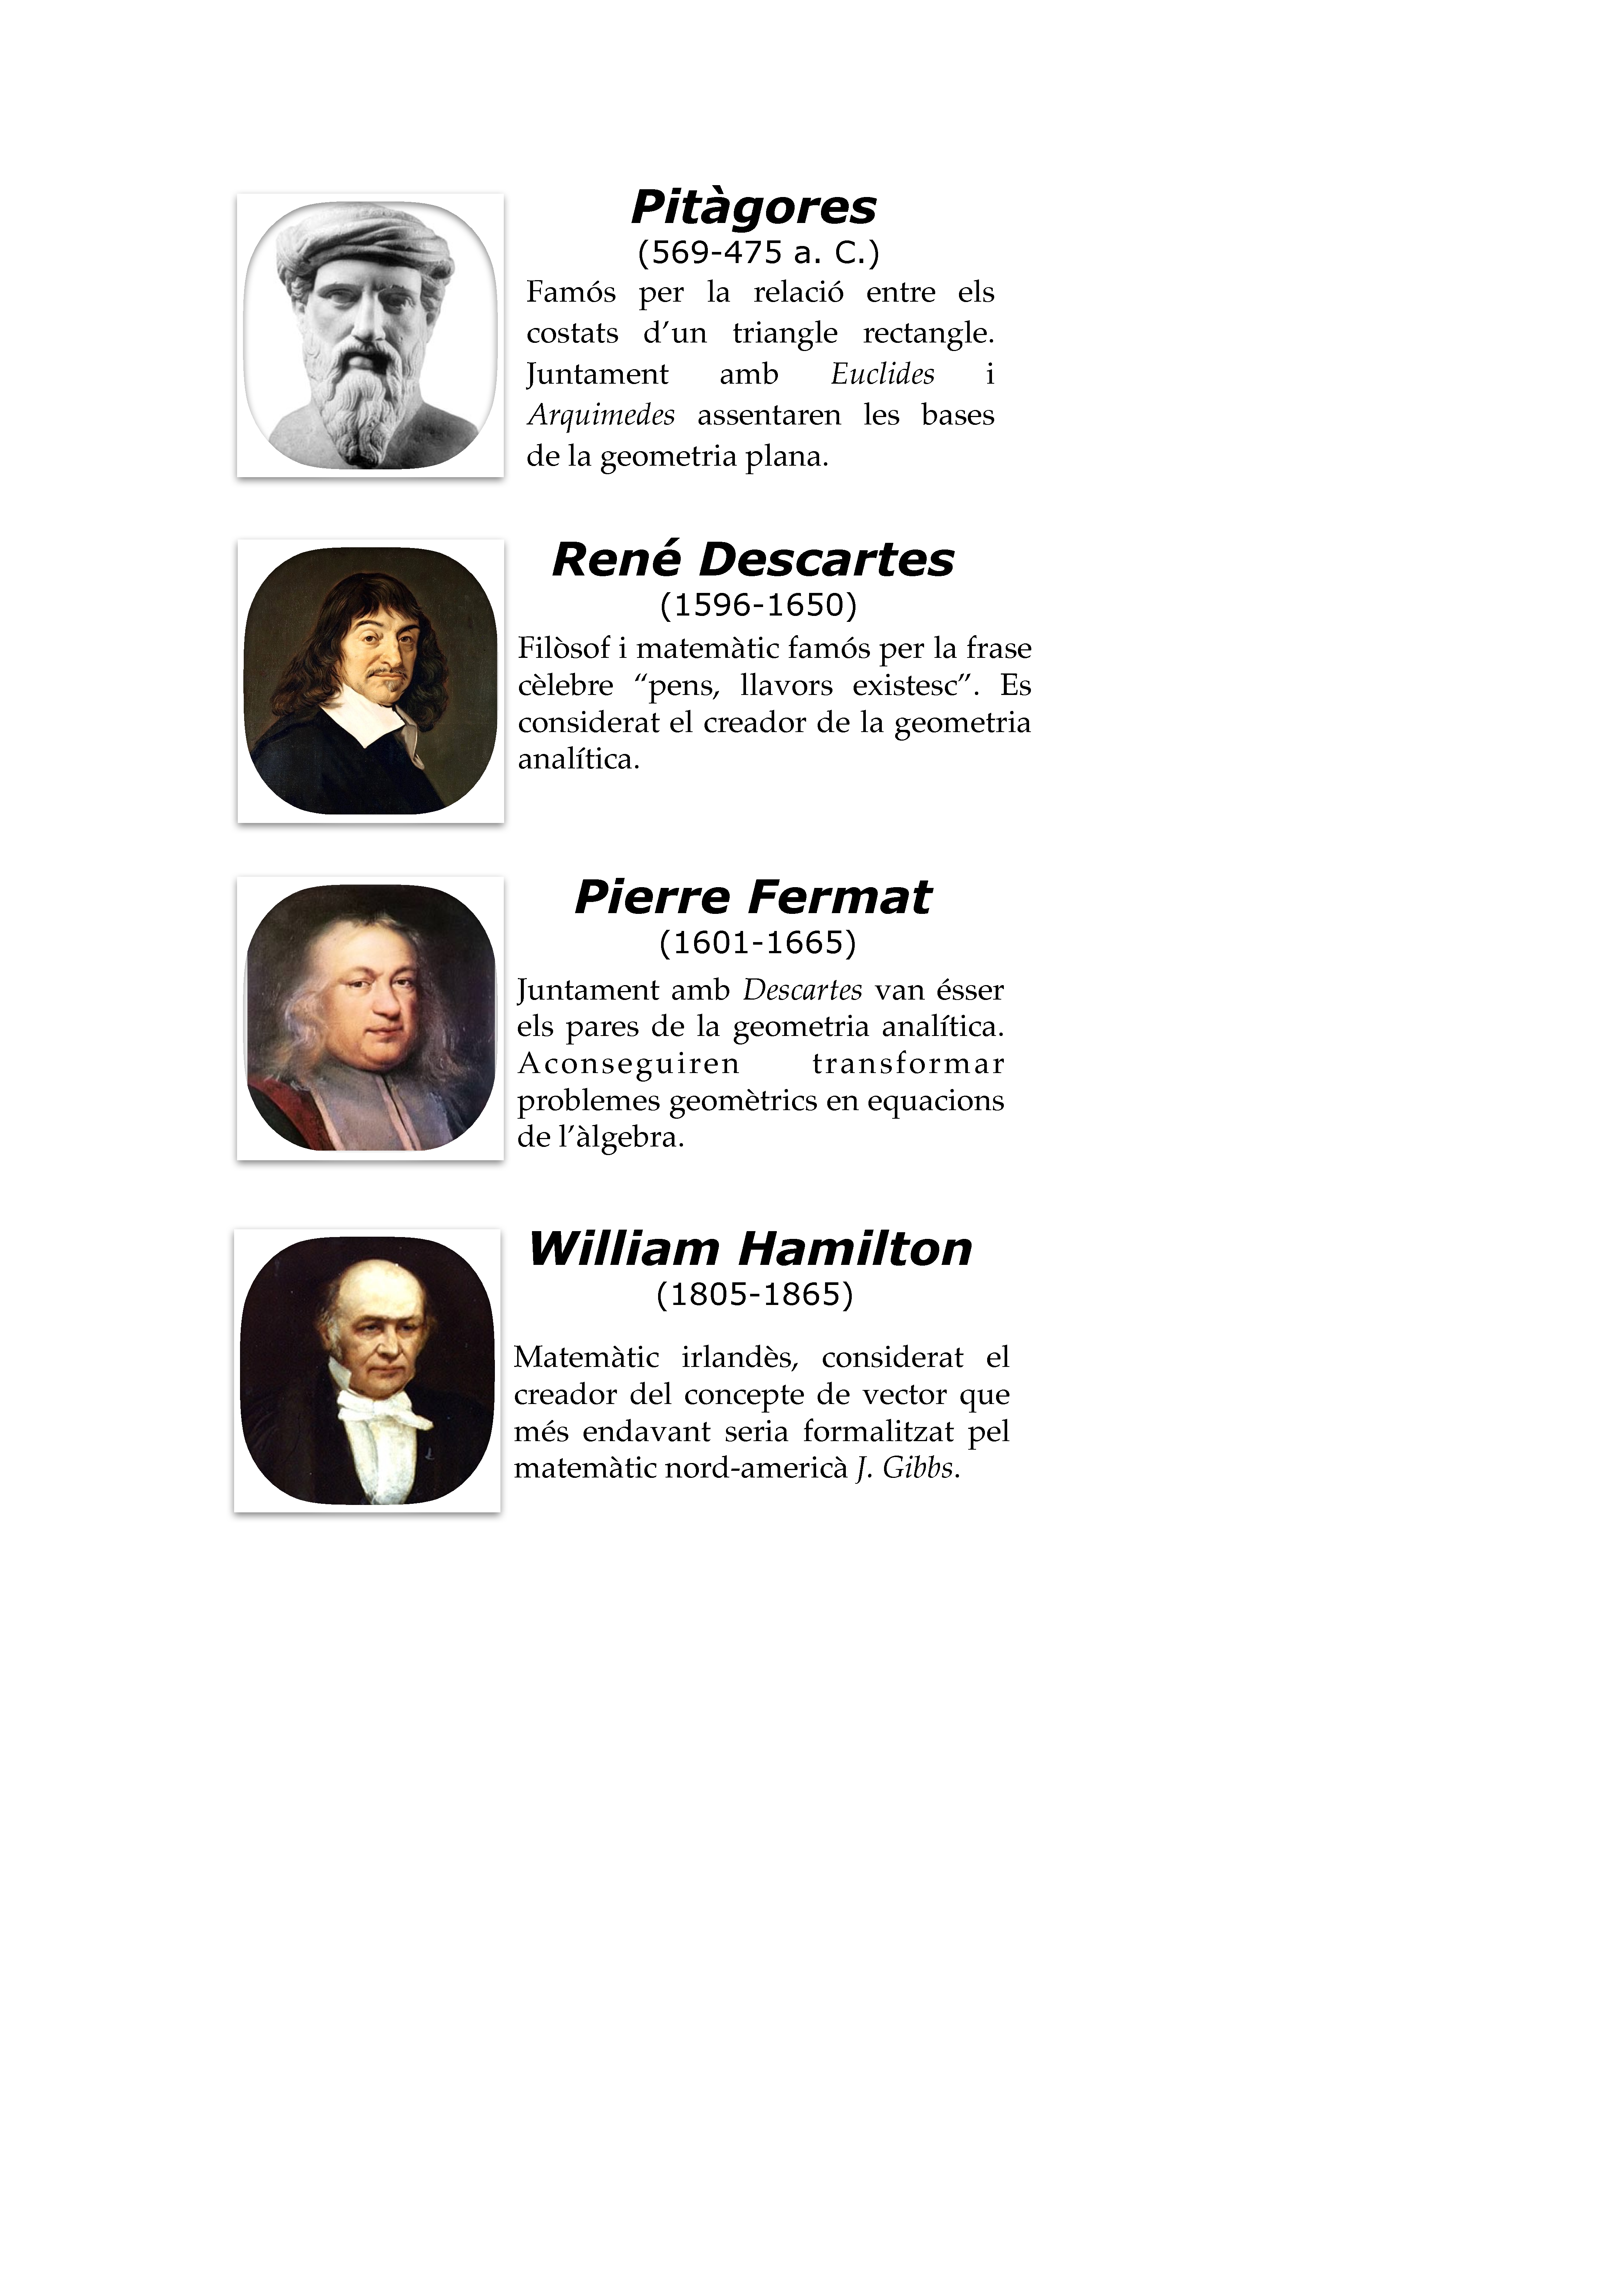
\includegraphics[width=0.65\textwidth]{img2/bloc3-historia}
\end{center}
\vspace*{\fill}

\include{chap-vectors}
\include{chap-analitica}
\include{chap-coniques}

%%%%% Activitats de bloc 3

\include{bloc3}
 
\mypart[(...) Aconseguírem obtenir així la fórmula estadística per conèixer la posició d'un electró. Però, personalment, no crec que Déu jugui als daus. --Albert Einstein--]{ESTADÍSTICA I PROBABILITAT}{img2/bloc4}

\vspace*{\fill}
\begin{center}
	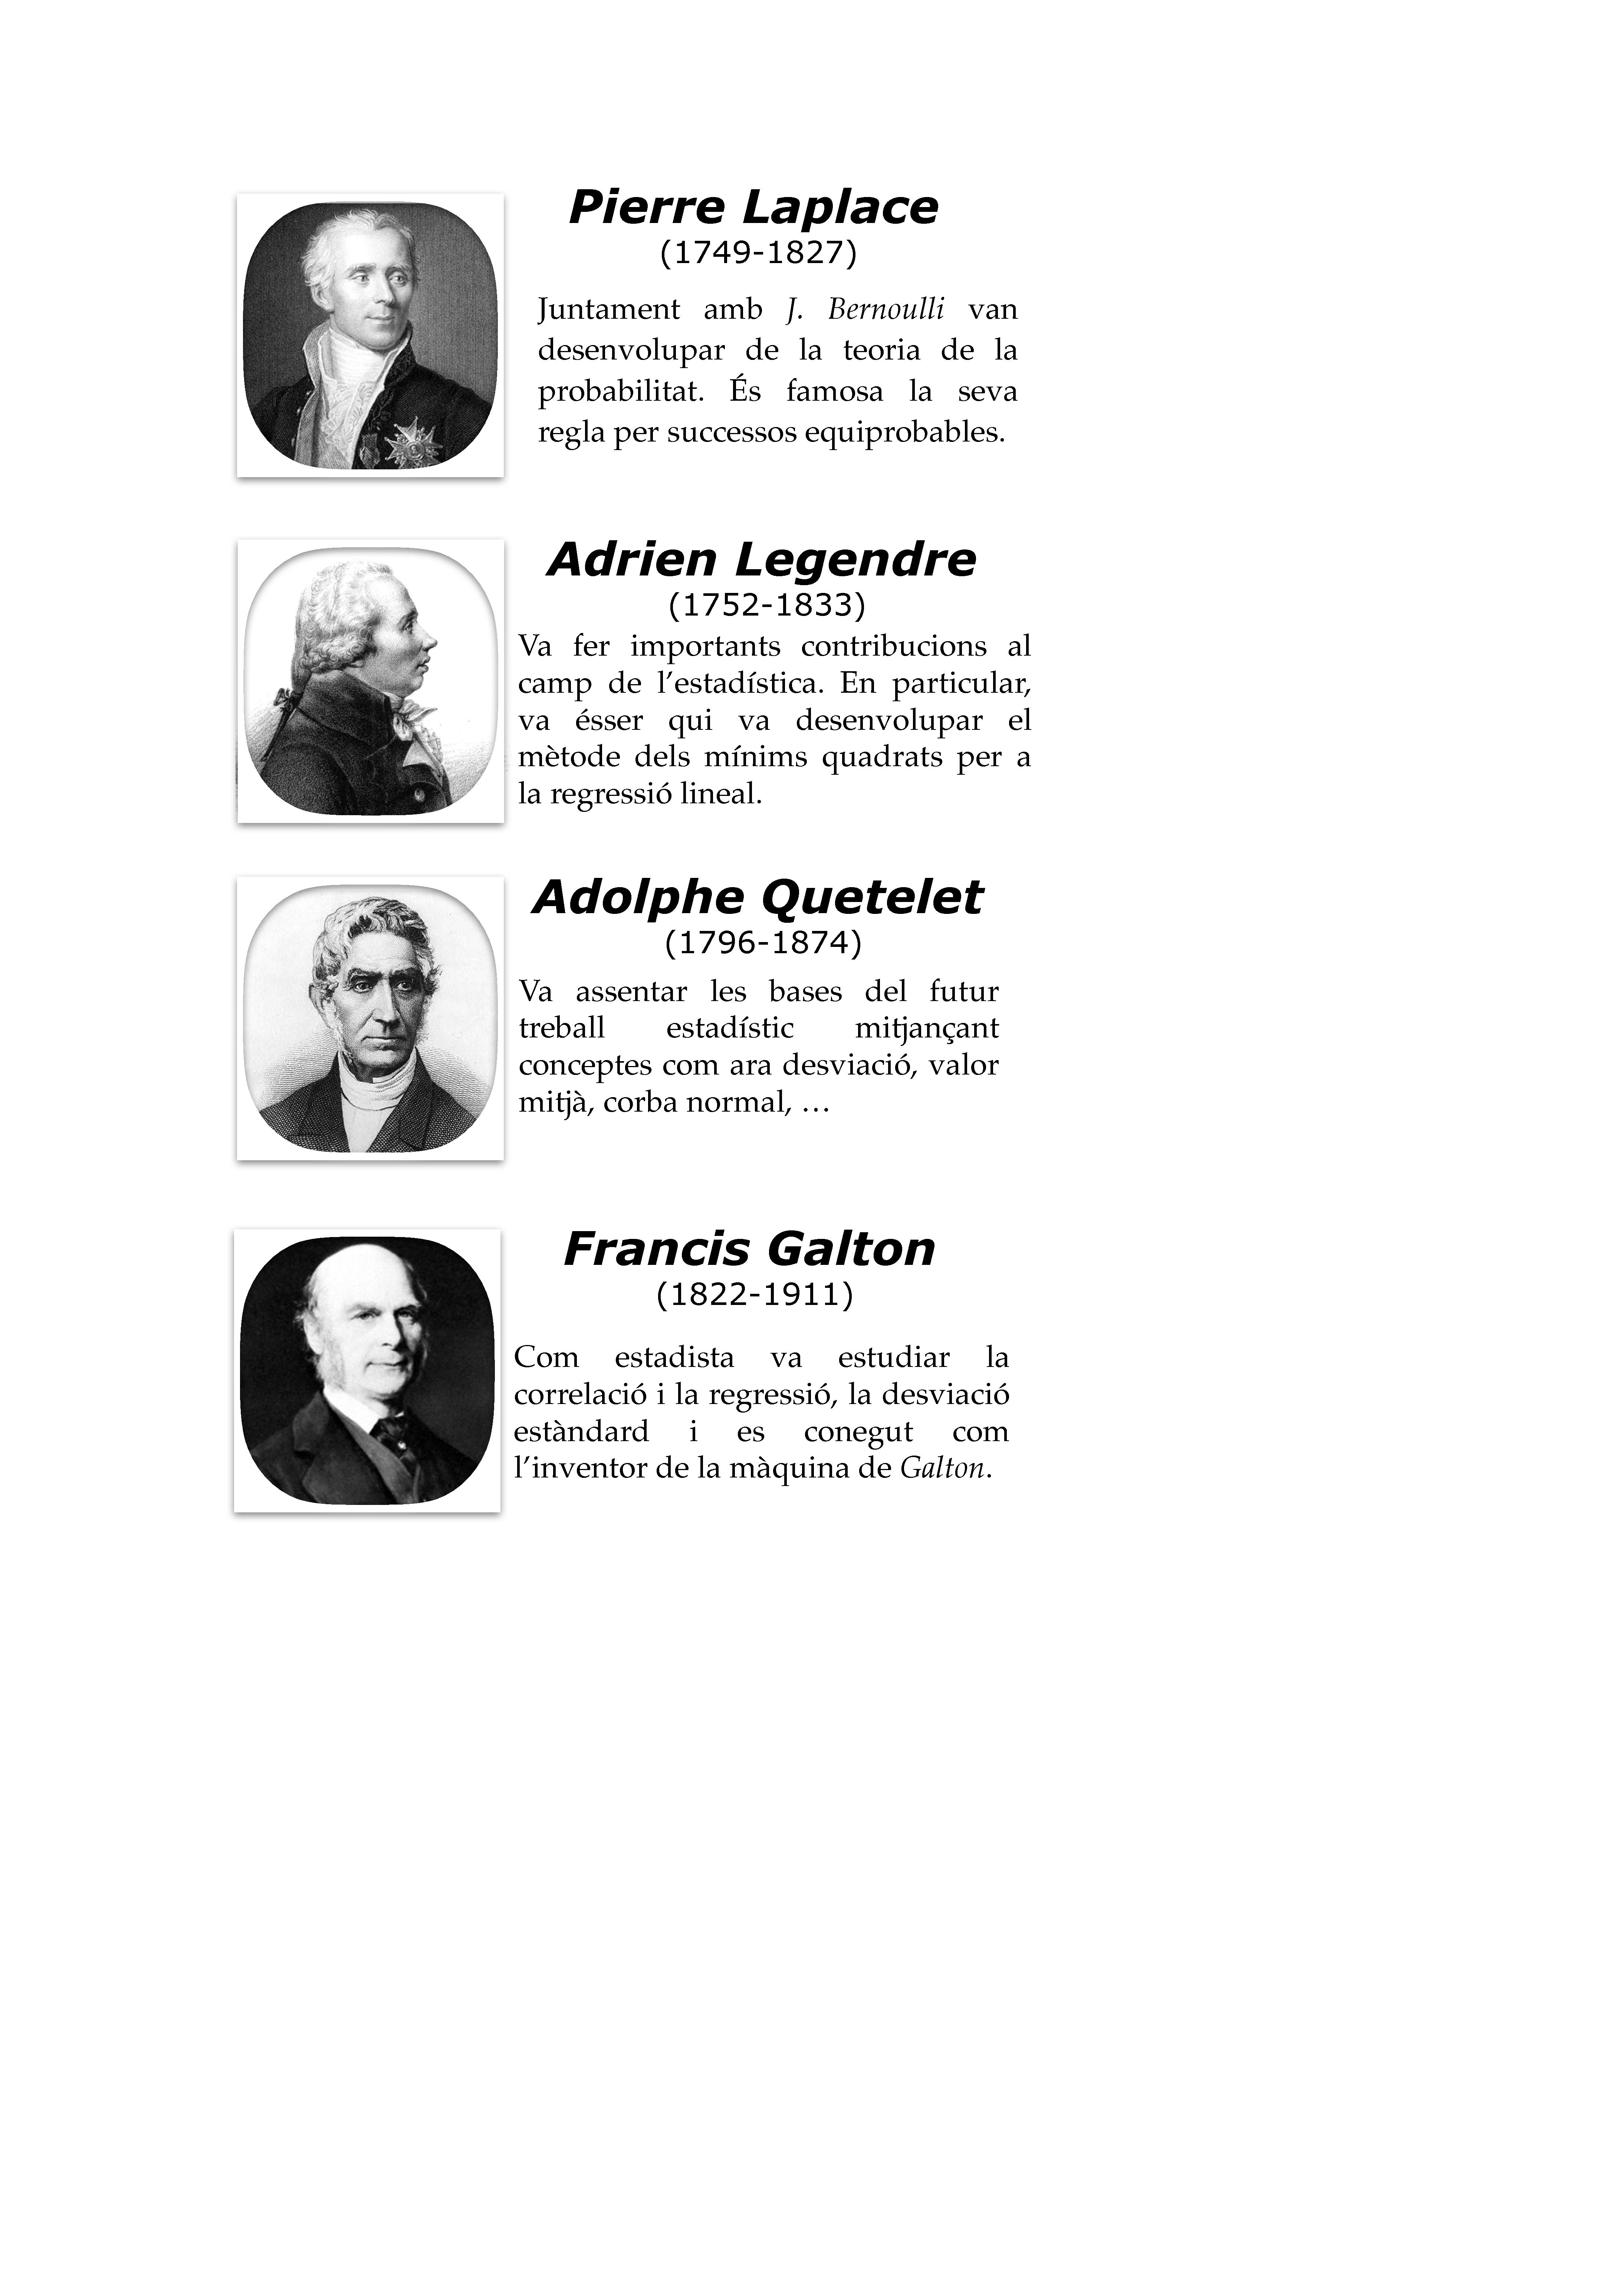
\includegraphics[width=0.65\textwidth]{img2/bloc4-historia}
\end{center}
\vspace*{\fill}

\include{chap-estadistica}

%\include{chap-probabilitat}


\pagestyle{blocfancy}

\newpage 
\immediate\closeout\studentkeys

\def\currentname{Solucionari}
\fakechapter[\simbolclaubig]{ Solucions }
\addcontentsline{toc}{part}{Solucions}
\begin{multicols}{2}
	\fontsize{10.5}{12.6}\selectfont
	
 \vspace{1cm} 
 
 \needspace{5\baselineskip} 
 \heading{Solucions del Tema 1}

\vspace{0.3cm}

 \needspace{3\baselineskip} 

\hyperlink{page.12}{\textbf{\em Pàgina 12}}
\begin{enumerate}


 \needspace{2\baselineskip} 

\phantomsection
 \item[\fontfamily{phv}\selectfont\color{blue}\textbf{\ref{exer:18}. }] \label{ans:18}
 \begin{tasks}[column-sep=1em, item-indent=1.3333em](3)
	 \task $\sqrt [{6}]{5} $
	 \task $\sqrt [{8}]{8} $
	 \task $\sqrt [{8}]{x^{7} } $
\end{tasks}
 \end{enumerate}
\begin{enumerate}


 \needspace{2\baselineskip} 

\phantomsection
 \item[\fontfamily{phv}\selectfont\color{blue}\textbf{\ref{exer:19}. }] \label{ans:19}
 \begin{tasks}[column-sep=1em, item-indent=1.3333em](3)
	 \task $2\,\sqrt [{}]{2} $
	 \task $9\,\sqrt [{}]{3} $
	 \task $\sqrt [{3}]{6} $
	 \task $2\,\sqrt [{4}]{2} $
	 \task $\sqrt [{3}]{3} $
	 \task $\sqrt [{3}]{49} $
	 \task $\sqrt [{8}]{7} $
	 \task $\sqrt {2} $
\end{tasks}


 \needspace{2\baselineskip} 

\phantomsection
 \item[\fontfamily{phv}\selectfont\color{blue}\textbf{\ref{exer:20}. }] \label{ans:20}
 \begin{tasks}[column-sep=1em, item-indent=1.3333em](2)
	 \task* $\sqrt [{4}]{2^{3} } =\sqrt [{12}]{2^{9} } $
	 \task* $\sqrt {7} =\sqrt [{16}]{7^{8} } $
	 \task* $\sqrt [{4}]{a^{6} } =\sqrt {a^{3} } $
	 \task* $\sqrt [{6}]{5^{12} } =\sqrt [{3}]{5^{6} } =5^{2} $
\end{tasks}
 \end{enumerate}
\vspace{0.3cm}

 \needspace{3\baselineskip} 

\hyperlink{page.13}{\textbf{\em Pàgina 13}}
\begin{enumerate}


 \needspace{2\baselineskip} 

\phantomsection
 \item[\fontfamily{phv}\selectfont\color{blue}\textbf{\ref{exer:21}. }] \label{ans:21}
 \begin{tasks}[column-sep=1em, item-indent=1.3333em](2)
	 \task $\sqrt [{3}]{5/4} $
	 \task $\sqrt [{12}]{2^{3} \cdot 3} $
	 \task $\sqrt [{12}]{5^{7} } $
	 \task $2^{3} $
	 \task $2^{4} \cdot \sqrt [{5}]{2^{4} } $
	 \task $\sqrt [{}]{5} $
	 \task 3
	 \task $5^{2} $
\end{tasks}
 \end{enumerate}
\begin{enumerate}


 \needspace{2\baselineskip} 

\phantomsection
 \item[\fontfamily{phv}\selectfont\color{blue}\textbf{\ref{exer:22}. }] \label{ans:22}
 \begin{tasks}[column-sep=1em, item-indent=1.3333em](3)
	 \task  $15\,\sqrt [{}]{11} $
	 \task $6\,\sqrt [{3}]{2} $
	 \task $-\sqrt [{}]{6} /5$
	 \task $-14\,\sqrt [{4}]{2} /3$
	 \task $41\,\sqrt [{}]{3} /15$
	 \task $13\,\sqrt [{}]{2} /5$
\end{tasks}
\phantomsection
\item[\fontfamily{phv}\selectfont\color{blue}\textbf{\ref{exer:23}. }] \label{ans:23} 
$(2+a)^{2} +4(2+a)\sqrt {a} +4a$


 \needspace{2\baselineskip} 

\phantomsection
 \item[\fontfamily{phv}\selectfont\color{blue}\textbf{\ref{exer:24}. }] \label{ans:24}
 \begin{tasks}[column-sep=1em, item-indent=1.3333em](2)
	 \task $\frac {\sqrt [{3}]{3^{2} } }{3} $
	 \task $\frac {3}{4} \,\sqrt [{4}]{2^{3} }$
	 \task $3(\sqrt {2+1} )$
	 \task $3+2\sqrt {2} $
	 \task $(\sqrt {10} -\sqrt {6} )/2$
	 \task $-(9+4\sqrt {5} )$
\end{tasks}


 \needspace{2\baselineskip} 

\phantomsection
 \item[\fontfamily{phv}\selectfont\color{blue}\textbf{\ref{exer:25}. }] \label{ans:25}
 \begin{tasks}[column-sep=1em, item-indent=1.3333em](2)
	 \task $3\sqrt {6}$
	 \task* $\frac {\sqrt [{4}]{2^{3} } }{2} $
	 \task $\frac {\sqrt {3} }{2} $
	 \task 35
	 \task $2^{-64/15} $
	 \task $33/4-5\sqrt {2} $
\end{tasks}
 \end{enumerate}
\vspace{0.3cm}

 \needspace{3\baselineskip} 

\hyperlink{page.14}{\textbf{\em Pàgina 14}}
\begin{enumerate}
\phantomsection
\item[\fontfamily{phv}\selectfont\color{blue}\textbf{\ref{exer:27}. }] \label{ans:27} 
$x=-10$ i $x=4$
 \end{enumerate}
\begin{enumerate}
\phantomsection
\item[\fontfamily{phv}\selectfont\color{blue}\textbf{\ref{exer:28}. }] \label{ans:28} 
$\sqrt [8]{x^3}$
\phantomsection
\item[\fontfamily{phv}\selectfont\color{blue}\textbf{\ref{exer:29}. }] \label{ans:29} 
$13+4\sqrt {3}$
\phantomsection
\item[\fontfamily{phv}\selectfont\color{blue}\textbf{\ref{exer:30}. }] \label{ans:30} 
$\dfrac {4\sqrt {5}}{5}$
\phantomsection
\item[\fontfamily{phv}\selectfont\color{blue}\textbf{\ref{exer:31}. }] \label{ans:31} 
$\frac {13}{3}\sqrt [3]{2}$
\phantomsection
\item[\fontfamily{phv}\selectfont\color{blue}\textbf{\ref{exer:32}. }] \label{ans:32} 
$\dfrac {16-5\sqrt {15}}{-7}$
\phantomsection
\item[\fontfamily{phv}\selectfont\color{blue}\textbf{\ref{exer:33}. }] \label{ans:33} 
$(-1,\,6]$
 \end{enumerate}

 \vspace{1cm} 
 
 \needspace{5\baselineskip} 
 \heading{Solucions del Tema 2}

\vspace{0.3cm}

 \needspace{3\baselineskip} 

\hyperlink{page.17}{\textbf{\em Pàgina 17}}
\begin{enumerate}


 \needspace{2\baselineskip} 

\phantomsection
 \item[\fontfamily{phv}\selectfont\color{blue}\textbf{\ref{exer:37}. }] \label{ans:37}
 \begin{tasks}[column-sep=1em, item-indent=1.3333em](1)
	 \task*  $Q(x)=3x^{3}+4x^{2}-x+2$; $R(x)=-4$
	 \task $Q(x)=2x+2$; $R(x)=2x-1$
	 \task* $Q(x)=a(x^{3}+ x^{2}+ x+ 1)$; $R(x)=a+b$
	 \task* $Q(x)=x^{8}+ x^{6}+ x^{4}+ x^{2}+ 1$; $R(x)=0$ 
\end{tasks}
 \end{enumerate}
\vspace{0.3cm}

 \needspace{3\baselineskip} 

\hyperlink{page.19}{\textbf{\em Pàgina 19}}
\begin{enumerate}


 \needspace{2\baselineskip} 

\phantomsection
 \item[\fontfamily{phv}\selectfont\color{blue}\textbf{\ref{exer:45}. }] \label{ans:45}
 \begin{tasks}[column-sep=1em, item-indent=1.3333em](1)
	 \task  $3(x+2)\cdot (x+1)$
	 \task $x^{3}\cdot (x+3)\cdot (x-3)$
	 \task $4(x+3)\cdot (x+1)\cdot (x-1)$
	 \task $-2(x+1)^{2}\cdot (x-3)$
	 \task $x\cdot (x^{3}-x^{2}+8x-4)$
	 \task ($x+1)^{2}\cdot (x-2)$
	 \task $2(x+1)\cdot (x-2)\cdot (x-5)$
	 \task $x^{2}\cdot (x+1)\cdot (x-3)$
	 \task $(x+4)\cdot (x+1)\cdot (x-2)$ 
\end{tasks}
 \end{enumerate}
\vspace{0.3cm}

 \needspace{3\baselineskip} 

\hyperlink{page.20}{\textbf{\em Pàgina 20}}
\begin{enumerate}


 \needspace{2\baselineskip} 

\phantomsection
 \item[\fontfamily{phv}\selectfont\color{blue}\textbf{\ref{exer:50}. }] \label{ans:50}
 \begin{tasks}[column-sep=1em, item-indent=1.3333em](1)
	 \task  $\dfrac {x-1}{3x(x+2)} $
	 \task $\dfrac {2(x+5)}{(x+1)^{2} } $
	 \task $\dfrac {x-1}{x(x+2)} $
	 \task \textit {No es pot}
	 \task* $\dfrac {(x^{2} +x+1)(x-1)}{x^{} } $
	 \task $\dfrac {1}{x+2} $
	 \task $\dfrac {x+2}{x-1} $
	 \task* $\dfrac {2(x^{4} -x^{3} +x^{2} -x+1)}{x} $
\end{tasks}
 \end{enumerate}
\vspace{0.3cm}

 \needspace{3\baselineskip} 

\hyperlink{page.21}{\textbf{\em Pàgina 21}}
\begin{enumerate}


 \needspace{2\baselineskip} 

\phantomsection
 \item[\fontfamily{phv}\selectfont\color{blue}\textbf{\ref{exer:54}. }] \label{ans:54}
 \begin{tasks}[column-sep=1em, item-indent=1.3333em](2)
	 \task  $\dfrac {-4x}{(x+1)(x-1)} $
	 \task $\dfrac {-2}{x+1} $
	 \task $\dfrac {-1}{x-1} $
	 \task $\dfrac {-2t+3}{t(t+2)} $
	 \task 0
	 \task $\dfrac {1-x^{2} }{x^{2} } $
	 \task $\dfrac {3x^{2} +5}{x(x+1)^{2} } $
\end{tasks}
 \end{enumerate}
\vspace{0.3cm}

 \needspace{3\baselineskip} 

\hyperlink{page.22}{\textbf{\em Pàgina 22}}
\begin{enumerate}


 \needspace{2\baselineskip} 

\phantomsection
 \item[\fontfamily{phv}\selectfont\color{blue}\textbf{\ref{exer:58}. }] \label{ans:58}
 \begin{tasks}[column-sep=1em, item-indent=1.3333em](2)
	 \task  $x=1,\,2,\,-2$
	 \task $x=0,\,5,\,-5$
	 \task $x=1,\,-2$
	 \task $x=\pm 2,\,3,\,-1$
	 \task $x=1,\,3,\,5,\,-4$
	 \task $x=1$
	 \task $x=-2,\,-1,\,2$
	 \task $x=-3,\,-1,\,2$
	 \task $x=-2,\,2,\,4$
	 \task $x=-3,\,-2,\,1$
	 \task $x=-3,\,3,\,-2,\,2$
	 \task $x=-1,\,0,\,5$ 
\end{tasks}
 \end{enumerate}
\vspace{0.3cm}

 \needspace{3\baselineskip} 

\hyperlink{page.23}{\textbf{\em Pàgina 23}}
\begin{enumerate}


 \needspace{2\baselineskip} 

\phantomsection
 \item[\fontfamily{phv}\selectfont\color{blue}\textbf{\ref{exer:64}. }] \label{ans:64}
 \begin{tasks}[column-sep=1em, item-indent=1.3333em](2)
	 \task  $x= \dfrac {2}{3},\,-\dfrac {1}{2}$
	 \task $x=2,\,\dfrac {1}{7}$
	 \task $x=2,\,-\dfrac {3}{5}$
	 \task $\dfrac {1\pm \sqrt {41}}{4}$
\end{tasks}
 \end{enumerate}
\begin{enumerate}


 \needspace{2\baselineskip} 

\phantomsection
 \item[\fontfamily{phv}\selectfont\color{blue}\textbf{\ref{exer:66}. }] \label{ans:66}
 \begin{tasks}[column-sep=1em, item-indent=1.3333em](2)
	 \task  $x=4$
	 \task $x=4$
	 \task $x=9$
	 \task $x=7$
	 \task $x=2$
	 \task $x=38414$
	 \task $x=10$
	 \task $x=3$
	 \task $x=11$
	 \task $x=29$
	 \task $x=14$
	 \task $x=1$
\end{tasks}
 \end{enumerate}
\vspace{0.3cm}

 \needspace{3\baselineskip} 

\hyperlink{page.24}{\textbf{\em Pàgina 24}}
\begin{enumerate}


 \needspace{2\baselineskip} 

\phantomsection
 \item[\fontfamily{phv}\selectfont\color{blue}\textbf{\ref{exer:67}. }] \label{ans:67}
 \begin{tasks}[column-sep=1em, item-indent=1.3333em](2)
	 \task  $x=1; y=16$
	 \task $x=6; y=8$
	 \task $x=10; y=2$
	 \task $x=4; y=7$
	 \task $x=3; y=1$
	 \task $x=-2; y=8$ 
\end{tasks}
 \end{enumerate}
\begin{enumerate}


 \needspace{2\baselineskip} 

\phantomsection
 \item[\fontfamily{phv}\selectfont\color{blue}\textbf{\ref{exer:69}. }] \label{ans:69}
 \begin{tasks}[column-sep=1em, item-indent=1.3333em](1)
	 \task  $x=7; y=2; z=11$
	 \task $x=4; y=-3; z=0$
	 \task $x=-1; y=4; z=4$
	 \task $x=8; y=4; z=-3$ 
\end{tasks}


 \needspace{2\baselineskip} 

\phantomsection
 \item[\fontfamily{phv}\selectfont\color{blue}\textbf{\ref{exer:70}. }] \label{ans:70}
 \begin{tasks}[column-sep=1em, item-indent=1.3333em](1)
	 \task  $x=1; y=-5; z=4$
	 \task $x=-1; y=-2; z=-2$
	 \task $x=15; y=2; z=1$
	 \task $x=3; y=4; z=9$ 
\end{tasks}
 \end{enumerate}
\vspace{0.3cm}

 \needspace{3\baselineskip} 

\hyperlink{page.25}{\textbf{\em Pàgina 25}}
\begin{enumerate}


 \needspace{2\baselineskip} 

\phantomsection
 \item[\fontfamily{phv}\selectfont\color{blue}\textbf{\ref{exer:71}. }] \label{ans:71}
 \begin{tasks}[column-sep=1em, item-indent=1.3333em](1)
	 \task  $x=1; y=-2; z=3$
	 \task $x=4; y=2; z=-3$
	 \task $x=1; y=-1; z=0$
	 \task $x=2; y=\dfrac {1}{5}; z=-1$ 
\end{tasks}
 \end{enumerate}
\vspace{0.3cm}

 \needspace{3\baselineskip} 

\hyperlink{page.28}{\textbf{\em Pàgina 28}}
\begin{enumerate}
\phantomsection
\item[\fontfamily{phv}\selectfont\color{blue}\textbf{\ref{exer:89}. }] \label{ans:89} 
$-3$
 \end{enumerate}
\begin{enumerate}
\phantomsection
\item[\fontfamily{phv}\selectfont\color{blue}\textbf{\ref{exer:90}. }] \label{ans:90} 
$Q=x^3$; $R=1$
\phantomsection
\item[\fontfamily{phv}\selectfont\color{blue}\textbf{\ref{exer:91}. }] \label{ans:91} 
No, si és de grau 4 pot tenir 4 arrels, que poden esser 4 reals, o be 2 arrels reals i 2 complexes o totes 4 complexes.
\phantomsection
\item[\fontfamily{phv}\selectfont\color{blue}\textbf{\ref{exer:92}. }] \label{ans:92} 
$x \in [-2, 2]$
\phantomsection
\item[\fontfamily{phv}\selectfont\color{blue}\textbf{\ref{exer:93}. }] \label{ans:93} 
$[-1, 15]$
\phantomsection
\item[\fontfamily{phv}\selectfont\color{blue}\textbf{\ref{exer:94}. }] \label{ans:94} 
$x \geq 9/5$ 
\phantomsection
\item[\fontfamily{phv}\selectfont\color{blue}\textbf{\ref{exer:95}. }] \label{ans:95} 
$x\in (1,2)$


 \needspace{2\baselineskip} 

\phantomsection
 \item[\fontfamily{phv}\selectfont\color{blue}\textbf{\ref{exer:96}. }] \label{ans:96}
 \begin{tasks}[column-sep=1em, item-indent=1.3333em](4)
	 \task F
	 \task V
	 \task F
	 \task F
\end{tasks}
 \end{enumerate}

 \vspace{1cm} 
 
 \needspace{5\baselineskip} 
 \heading{Solucions del Tema 3}

\vspace{0.3cm}

 \needspace{3\baselineskip} 

\hyperlink{page.33}{\textbf{\em Pàgina 33}}
\begin{enumerate}


 \needspace{2\baselineskip} 

\phantomsection
 \item[\fontfamily{phv}\selectfont\color{blue}\textbf{\ref{exer:110}. }] \label{ans:110}
 \begin{tasks}[column-sep=1em, item-indent=1.3333em](1)
	 \task* $\hat C=33$; $b=26,8$; $c=17,4$
	 \task* $\hat B=67$; $b=66,3$; $c=28,1$
	 \task* $\hat C=39$; $\hat B=51$; $a=396,7$
	 \task* $\hat B=58$; $b=56,01$; $a=66,05$
\end{tasks}
 \end{enumerate}
\begin{enumerate}
\phantomsection
\item[\fontfamily{phv}\selectfont\color{blue}\textbf{\ref{exer:111}. }] \label{ans:111} 
$a=3,46$; $b=1,73$
\phantomsection
\item[\fontfamily{phv}\selectfont\color{blue}\textbf{\ref{exer:112}. }] \label{ans:112} 
$\alpha =25,5^\circ $
\phantomsection
\item[\fontfamily{phv}\selectfont\color{blue}\textbf{\ref{exer:113}. }] \label{ans:113} 
 $a=25$; $c=20$; $\hat B=36,87^\circ $; $\hat C=53,13^\circ $
 \end{enumerate}
\vspace{0.3cm}

 \needspace{3\baselineskip} 

\hyperlink{page.37}{\textbf{\em Pàgina 37}}
\begin{enumerate}
\phantomsection
\item[\fontfamily{phv}\selectfont\color{blue}\textbf{\ref{exer:140}. }] \label{ans:140} 
$d=35,49$ km
 \end{enumerate}
\vspace{0.3cm}

 \needspace{3\baselineskip} 

\hyperlink{page.38}{\textbf{\em Pàgina 38}}
\begin{enumerate}
\phantomsection
\item[\fontfamily{phv}\selectfont\color{blue}\textbf{\ref{exer:141}. }] \label{ans:141} 
Del triangle $\widehat {CAD}$ troba $\overline {AD}=74.16$ km, del triangle $\widehat {CBD}$ troba $\overline {BD}=52.05$ km pel teorema del sinus i finalment del triangle $\widehat {ADB}$ troba $\overline {AB}=24$ km pel teorema del cosinus.
 \end{enumerate}
\begin{enumerate}
\phantomsection
\item[\fontfamily{phv}\selectfont\color{blue}\textbf{\ref{exer:142}. }] \label{ans:142} 
cim A=827 m, cim B=751 m, distància entre cims AB=1687.3 m
 \end{enumerate}
\vspace{0.3cm}

 \needspace{3\baselineskip} 

\hyperlink{page.39}{\textbf{\em Pàgina 39}}
\begin{enumerate}
\phantomsection
\item[\fontfamily{phv}\selectfont\color{blue}\textbf{\ref{exer:150}. }] \label{ans:150} 
Treu factor comú $\cos \alpha $ i utilitza la relació fonamental.
 \end{enumerate}
\begin{enumerate}
\phantomsection
\item[\fontfamily{phv}\selectfont\color{blue}\textbf{\ref{exer:151}. }] \label{ans:151} 
Desenvolupa el quadrat amb la identitat notable $(a+b)^2 = a^2 + b^2 + 2ab$. Empra la relació fonamental i la fórmula de $\sin 2\alf $.
\phantomsection
\item[\fontfamily{phv}\selectfont\color{blue}\textbf{\ref{exer:152}. }] \label{ans:152} 
Utilitza les relacions de l'angle oposat $\cos (-x)=\cos x$, $\sin (-x)=-\sin x$, $\tg (-x)=-\tg x$.
\phantomsection
\item[\fontfamily{phv}\selectfont\color{blue}\textbf{\ref{exer:153}. }] \label{ans:153} 
Expressa $\tg \alf $ i $\cotg \alf $ com a quocients de sinus i cosinus. Després realitza la suma de fraccions amb el mínim comú múltiple. Finalment utilitza la relació fonamental.
\phantomsection
\item[\fontfamily{phv}\selectfont\color{blue}\textbf{\ref{exer:154}. }] \label{ans:154} 
Escriu $\sin (3\alf ) = \sin (\alf +2\alf )$. Aplica la fórmula de la suma d'angles i tot seguit les fórmules de l'angle doble. Finalment opera, simplifica i treu factor comú $\sin \alf $.
\phantomsection
\item[\fontfamily{phv}\selectfont\color{blue}\textbf{\ref{exer:155}. }] \label{ans:155} 
Escriu $\cos (4\alf ) = \cos (2\alf +2\alf )$. Aplica la fórmula de la suma d'angles i tot seguit les fórmules de l'angle doble. Finalment opera i simplifica.
 \end{enumerate}
\vspace{0.3cm}

 \needspace{3\baselineskip} 

\hyperlink{page.42}{\textbf{\em Pàgina 42}}
\begin{enumerate}


 \needspace{2\baselineskip} 

\phantomsection
 \item[\fontfamily{phv}\selectfont\color{blue}\textbf{\ref{exer:172}. }] \label{ans:172}
 \begin{tasks}[column-sep=1em, item-indent=1.3333em](1)
	 \task $\sin (-750^\circ )=1/2$
	 \task* $\tg 570^\circ =\frac {-1}{\sqrt 3}=-\frac {\sqrt 3}{3}$
	 \task $\cos 20\pi /3 = -1/2$
\end{tasks}
 \end{enumerate}
\begin{enumerate}
\phantomsection
\item[\fontfamily{phv}\selectfont\color{blue}\textbf{\ref{exer:173}. }] \label{ans:173} 
$\sin (105)=\sin (60+45)=\frac {\sqrt {6}+\sqrt {2}}{4}$ \par $\cos (75)=\sin (30+45)=\frac {\sqrt {6}-\sqrt {2}}{4}$
\phantomsection
\item[\fontfamily{phv}\selectfont\color{blue}\textbf{\ref{exer:174}. }] \label{ans:174} 
$c=17,32$, $\hat B=90^\circ $, $\hat C=60^\circ $
\phantomsection
\item[\fontfamily{phv}\selectfont\color{blue}\textbf{\ref{exer:175}. }] \label{ans:175} 
Sí ho aconseguirà. Estan a 105,83 m.
\phantomsection
\item[\fontfamily{phv}\selectfont\color{blue}\textbf{\ref{exer:176}. }] \label{ans:176} 
$\sin a=\frac {-1}{\sqrt 5}=-\frac {\sqrt 5}{5}$\par $\cos a=\frac {-2}{\sqrt 5}=-\frac {2\sqrt 5}{5}$;
\phantomsection
\item[\fontfamily{phv}\selectfont\color{blue}\textbf{\ref{exer:177}. }] \label{ans:177} 
a) $x=\left \{\begin {array}{l} 120 + n 360 \\ 240 +n 360 \end {array}\right .$ \par b) $x=45 + n 180$
\phantomsection
\item[\fontfamily{phv}\selectfont\color{blue}\textbf{\ref{exer:178}. }] \label{ans:178} 
a) $(60+360k,120–360k)$ i \par $(120+360k,60–360k)$; \par b) $(75+360k, 15–360k)$ i \par $(15+360k, 75–360k)$
\phantomsection
\item[\fontfamily{phv}\selectfont\color{blue}\textbf{\ref{exer:179}. }] \label{ans:179} 
Substituir el $\sin (2a)$ pel seu valor i aplicar que $1–\cos 2a$ és el sinus al quadrat.
\phantomsection
\item[\fontfamily{phv}\selectfont\color{blue}\textbf{\ref{exer:180}. }] \label{ans:180} 
Perímetre = $300\cdot \sin 36^\circ = 176,3355$ m.; \quad Àrea = 713,292 m$^2$.
\phantomsection
\item[\fontfamily{phv}\selectfont\color{blue}\textbf{\ref{exer:181}. }] \label{ans:181} 
$8,63^\circ $
 \end{enumerate}

 \vspace{1cm} 
 
 \needspace{5\baselineskip} 
 \heading{Solucions del Tema 4}

\vspace{0.3cm}

 \needspace{3\baselineskip} 

\hyperlink{page.48}{\textbf{\em Pàgina 48}}
\begin{enumerate}


 \needspace{2\baselineskip} 

\phantomsection
 \item[\fontfamily{phv}\selectfont\color{blue}\textbf{\ref{exer:183}. }] \label{ans:183}
 \begin{tasks}[column-sep=1em, item-indent=1.3333em](2)
	 \task  $5 -9i$
	 \task $-6-15i$
	 \task $-13+11i$
	 \task 0
	 \task 13
	 \task $4 + 10i$
	 \task $2i$
	 \task $-4$
\end{tasks}
 \end{enumerate}
\begin{enumerate}


 \needspace{2\baselineskip} 

\phantomsection
 \item[\fontfamily{phv}\selectfont\color{blue}\textbf{\ref{exer:184}. }] \label{ans:184}
 \begin{tasks}[column-sep=1em, item-indent=1.3333em](2)
	 \task  $-{{1}\over {10}}-{{7\,i}\over {10}}$
	 \task $-{{11}\over {6}}+{{i}\over {2}}$
	 \task ${{2}\over {5}}-{{i}\over {5}}$
	 \task ${{34\,i}\over {5}}$
\end{tasks}


 \needspace{2\baselineskip} 

\phantomsection
 \item[\fontfamily{phv}\selectfont\color{blue}\textbf{\ref{exer:187}. }] \label{ans:187}
 \begin{tasks}[column-sep=1em, item-indent=1.3333em](1)
	 \task  $|z|=2$; $arg(z)=-30^\circ $
	 \task* $|z|=\sqrt {8}$; $arg(z)=225 = - 135^\circ $
	 \task $|z|=2$; $arg(z)=-60^\circ $
	 \task $|z|=4$; $arg(z)=-90^\circ $
\end{tasks}
 \end{enumerate}
\vspace{0.3cm}

 \needspace{3\baselineskip} 

\hyperlink{page.49}{\textbf{\em Pàgina 49}}
\begin{enumerate}


 \needspace{2\baselineskip} 

\phantomsection
 \item[\fontfamily{phv}\selectfont\color{blue}\textbf{\ref{exer:192}. }] \label{ans:192}
 \begin{tasks}[column-sep=1em, item-indent=1.3333em](1)
	 \task*  $2_{\,60^\circ }= 1 - \sqrt {3} i$
	 \task* $3_{\,-45^\circ }= \frac {3\sqrt {2}}{2} - \frac {3\sqrt {2}}{2} i$
	 \task $1_{\,90^\circ }= i $
	 \task* $5_{\,120^\circ }= -\frac {5}{2} + i \frac {5\sqrt {3}}{2}$
\end{tasks}
 \end{enumerate}
\vspace{0.3cm}

 \needspace{3\baselineskip} 

\hyperlink{page.52}{\textbf{\em Pàgina 52}}
\begin{enumerate}


 \needspace{2\baselineskip} 

\phantomsection
 \item[\fontfamily{phv}\selectfont\color{blue}\textbf{\ref{exer:206}. }] \label{ans:206}
 \begin{tasks}[column-sep=1em, item-indent=1.3333em](2)
	 \task $-5-6i$
	 \task $-8-6i$
	 \task $10i$
	 \task $-2+i$
\end{tasks}
 \end{enumerate}
\begin{enumerate}
\phantomsection
\item[\fontfamily{phv}\selectfont\color{blue}\textbf{\ref{exer:207}. }] \label{ans:207} 
$-46+63i$
\phantomsection
\item[\fontfamily{phv}\selectfont\color{blue}\textbf{\ref{exer:208}. }] \label{ans:208} 
$z_1=5+2i$, $z_2=5-2i$


 \needspace{2\baselineskip} 

\phantomsection
 \item[\fontfamily{phv}\selectfont\color{blue}\textbf{\ref{exer:209}. }] \label{ans:209}
 \begin{tasks}[column-sep=1em, item-indent=1.3333em](2)
	 \task Real $k=-2$
	 \task Imaginari pur $k=-2$
\end{tasks}
\phantomsection
\item[\fontfamily{phv}\selectfont\color{blue}\textbf{\ref{exer:210}. }] \label{ans:210} 
$x=\pm 2$
\phantomsection
\item[\fontfamily{phv}\selectfont\color{blue}\textbf{\ref{exer:211}. }] \label{ans:211} 
$3\sqrt {2}$, $3\pi /4$
\phantomsection
\item[\fontfamily{phv}\selectfont\color{blue}\textbf{\ref{exer:212}. }] \label{ans:212} 
$1+\sqrt {3}i$
\phantomsection
\item[\fontfamily{phv}\selectfont\color{blue}\textbf{\ref{exer:213}. }] \label{ans:213} 
$-8i$
\phantomsection
\item[\fontfamily{phv}\selectfont\color{blue}\textbf{\ref{exer:214}. }] \label{ans:214} 
$5(\cos (\pi /2) +i \sin (\pi /2)$
\phantomsection
\item[\fontfamily{phv}\selectfont\color{blue}\textbf{\ref{exer:215}. }] \label{ans:215} 
$z_1=2_{110^\circ }$, $z_2=2_{230^\circ }$, $z_3=2_{350^\circ }$
 \end{enumerate}

 \vspace{1cm} 

 \needspace{5\baselineskip} 
 \heading{Solucions del Bloc I}

\vspace{0.3cm}

 \needspace{3\baselineskip} 

\hyperlink{page.54}{\textbf{\em Pàgina 54}}
\begin{enumerate}
\phantomsection
\item[\fontfamily{phv}\selectfont\color{blue}\textbf{\ref{exer:216}. }] \label{ans:216} 
a) $a\sqrt {a}$ \quad \quad b) $\frac {3\sqrt {2}-4\sqrt {6}}{6}$
 \end{enumerate}
\begin{enumerate}
\phantomsection
\item[\fontfamily{phv}\selectfont\color{blue}\textbf{\ref{exer:217}. }] \label{ans:217} 
a) $a\,\sqrt [20]{a}$ \quad \quad b)$\frac {2\sqrt {3}+3\sqrt {2}-6}{6}$
\phantomsection
\item[\fontfamily{phv}\selectfont\color{blue}\textbf{\ref{exer:218}. }] \label{ans:218} 
$x^2 (x+1) (x-2) (3x-1)$
\phantomsection
\item[\fontfamily{phv}\selectfont\color{blue}\textbf{\ref{exer:219}. }] \label{ans:219} 
2
\phantomsection
\item[\fontfamily{phv}\selectfont\color{blue}\textbf{\ref{exer:220}. }] \label{ans:220} 
$x=3$ vàlida.
\phantomsection
\item[\fontfamily{phv}\selectfont\color{blue}\textbf{\ref{exer:221}. }] \label{ans:221} 
$x=1$
\phantomsection
\item[\fontfamily{phv}\selectfont\color{blue}\textbf{\ref{exer:222}. }] \label{ans:222} 
$(3, +\infty )$
\phantomsection
\item[\fontfamily{phv}\selectfont\color{blue}\textbf{\ref{exer:223}. }] \label{ans:223} 
$x=38$: be, $y=18$: malament, $z=4$: no contestades. Planteig: $x+y+z=60$; $5x-2y-z=150$; $y+5z=x$
\phantomsection
\item[\fontfamily{phv}\selectfont\color{blue}\textbf{\ref{exer:224}. }] \label{ans:224} 
S.C.I. $x=1$, $y=z-3$, $z=z$
 \end{enumerate}
\vspace{0.3cm}

 \needspace{3\baselineskip} 

\hyperlink{page.55}{\textbf{\em Pàgina 55}}
\begin{enumerate}
\phantomsection
\item[\fontfamily{phv}\selectfont\color{blue}\textbf{\ref{exer:225}. }] \label{ans:225} 
Els costats són 10.49 cm i 20.25 cm, el perímetre 61.48 cm. L'àrea 83.23 cm$^2$.
 \end{enumerate}
\begin{enumerate}
\phantomsection
\item[\fontfamily{phv}\selectfont\color{blue}\textbf{\ref{exer:226}. }] \label{ans:226} 
Primer obtenim els costats resolent un sistema d'equacions $a=19$, $b=16$ i $c=13$. Després aplicam el Teorema del Cosinus per obtenir els angles $\hat A=42.54^\circ $, $\hat B=56.3^\circ $, $\hat C=81.17^\circ $
\phantomsection
\item[\fontfamily{phv}\selectfont\color{blue}\textbf{\ref{exer:227}. }] \label{ans:227} 
Utilitzam el Teorema del Sinus. $\hat C= 56^\circ \, 19^\prime \, 31^{\prime \prime }$, $\hat B= 51^\circ \, 40^\prime \, 29^{\prime \prime }$ i $\bar {AC}=263.96$ m.
\phantomsection
\item[\fontfamily{phv}\selectfont\color{blue}\textbf{\ref{exer:228}. }] \label{ans:228} 
$d=3557$ km sobre la superfície de la Terra.
\phantomsection
\item[\fontfamily{phv}\selectfont\color{blue}\textbf{\ref{exer:229}. }] \label{ans:229} 
No existeix cap angle amb aquestes condicions. S'obtindria que $\cos a = 3/4$ i amb aquesta dada no es compleix que $\sin ^2 a +\cos ^2 a = 1$.
\phantomsection
\item[\fontfamily{phv}\selectfont\color{blue}\textbf{\ref{exer:230}. }] \label{ans:230} 
En primer lloc trobam que $\sin \alpha = \frac {2\sqrt 5}{5}$ i $\cos \alpha = \frac {\sqrt 5}{5}$. a) $-3/5$ \quad b) $\frac {\sqrt 5}{5}$ \quad c) $\sqrt {\frac {5-\sqrt 5}{10}}$ \quad d) $-3$
\phantomsection
\item[\fontfamily{phv}\selectfont\color{blue}\textbf{\ref{exer:231}. }] \label{ans:231} 
a) Utilitza que $sin^4 x = (1-\cos ^2 x)^2$ desenvolupa el quadrat i simplifica. b) Utilitza que $\cos ^2 \frac {\beta }{2} = \frac {1+\cos \beta }{2}$ 
\phantomsection
\item[\fontfamily{phv}\selectfont\color{blue}\textbf{\ref{exer:232}. }] \label{ans:232} 
a) $x= 0^\circ + n\cdot 360^\circ $, $x=126.87^\circ + n\cdot 360^\circ $. b) $x= 90^\circ + n\cdot 180^\circ $, $x= 60^\circ + n\cdot 360^\circ $, $x= 300^\circ + n\cdot 360^\circ $.
\phantomsection
\item[\fontfamily{phv}\selectfont\color{blue}\textbf{\ref{exer:233}. }] \label{ans:233} 
$x=30^\circ + n\cdot 180^\circ $, $y=30^\circ + k\cdot 180^\circ $.
\phantomsection
\item[\fontfamily{phv}\selectfont\color{blue}\textbf{\ref{exer:234}. }] \label{ans:234} 
$-\frac {19}{10}+\frac {37}{10}i$
\phantomsection
\item[\fontfamily{phv}\selectfont\color{blue}\textbf{\ref{exer:235}. }] \label{ans:235} 
$i$
\phantomsection
\item[\fontfamily{phv}\selectfont\color{blue}\textbf{\ref{exer:236}. }] \label{ans:236} 
$z=5+2i$, $z=5-2i$
\phantomsection
\item[\fontfamily{phv}\selectfont\color{blue}\textbf{\ref{exer:237}. }] \label{ans:237} 
 $z^*=3_{\, 300^\circ }$, $1/z=(1/3)_{\, 300^\circ }$, $z^2=9_{\, 120^\circ }$, $\sqrt [3]{z}$ té tres resultats = $(\sqrt {3})_{\, 20^\circ }$, $(\sqrt {3})_{\, 140^\circ }$ i $(\sqrt {3})_{\, 260^\circ }$.
 \end{enumerate}

 \vspace{1cm} 
 
 \needspace{5\baselineskip} 
 \heading{Solucions del Tema 5}

\vspace{0.3cm}

 \needspace{3\baselineskip} 

\hyperlink{page.60}{\textbf{\em Pàgina 60}}
\begin{enumerate}
\phantomsection
\item[\fontfamily{phv}\selectfont\color{blue}\textbf{\ref{exer:239}. }] \label{ans:239} 
2, 3, 5, 8, 13, 21, 34, ...
 \end{enumerate}
\begin{enumerate}
\phantomsection
\item[\fontfamily{phv}\selectfont\color{blue}\textbf{\ref{exer:240}. }] \label{ans:240} 
a) $a_n=3+5(n-1)$ o $a_1=3$ $a_n=a_{n-1}+3$ \par b) $a_n=n^3$ \par c) $a_n=8\cdot (1/2)^{n-1}$ o $a_1=8$ $a_n=a_{n-1}/2$]
\phantomsection
\item[\fontfamily{phv}\selectfont\color{blue}\textbf{\ref{exer:241}. }] \label{ans:241} 
$a_n=10-3(n-1)$ i $a_{100}=-197$
\phantomsection
\item[\fontfamily{phv}\selectfont\color{blue}\textbf{\ref{exer:242}. }] \label{ans:242} 
$d=(19-11)/2=4$ i $a_1=3$, \linebreak $a_n=3+4(n-1)$, $S_{100}=20100$
\phantomsection
\item[\fontfamily{phv}\selectfont\color{blue}\textbf{\ref{exer:243}. }] \label{ans:243} 
$a_n=100\cdot (0.5)^{n-1}$, $a_{50}=1.776\cdot 10^{-13}$, $S_\infty =200$
\phantomsection
\item[\fontfamily{phv}\selectfont\color{blue}\textbf{\ref{exer:244}. }] \label{ans:244} 
$r=3$ i $a_1=1$, $a_n=3^{n-1}$, $S_{30}=1.029\cdot 10^{14}$
 \end{enumerate}
\vspace{0.3cm}

 \needspace{3\baselineskip} 

\hyperlink{page.62}{\textbf{\em Pàgina 62}}
\begin{enumerate}
\phantomsection
\item[\fontfamily{phv}\selectfont\color{blue}\textbf{\ref{exer:247}. }] \label{ans:247} 
$\text {Dom }f=\Re -\{\pm 2\}$,\par $\text {Dom } g=(-\infty ,-2/3]\cup (3,+\infty )$,\par $\text {Dom } h=\Re -\{1\}$,\par $\text {Dom } i=\Re -\{\pm 1\}$,\par $\text {Dom } j=(-\infty ,-3]\cup (3,+\infty )$,\par $\text {Dom } k=\Re -\{\pm \sqrt {3}\}$,\par $\text {Dom } l=[-2,3)$, $\text {Dom } m=\Re - \{1\}$
 \end{enumerate}
\vspace{0.3cm}

 \needspace{3\baselineskip} 

\hyperlink{page.66}{\textbf{\em Pàgina 66}}
\begin{enumerate}
\phantomsection
\item[\fontfamily{phv}\selectfont\color{blue}\textbf{\ref{exer:271}. }] \label{ans:271} 
$p^{-1}=(3-x)/5$,\par $q^{-1}=\pm \sqrt {(x+1)/2}$,\par $r^{-1}=\sqrt [3]{6-x}$, $s^{-1}=-x$,\par $f^{-1}=(3x+4)/(2-x)$, $g^{-1}=-3/x$,\par $h^{-1}=(1\pm \sqrt {1+4x})/2$,\par $j^{-1}=\pm \sqrt {4x/(1+x)}$, \,\,$k^{-1}=4+\ln x$,\par $l^{-1}=1/\log _2 {x}$,\par $m^{-1}=\log x /(\log 2 - \log 3)$,\par $n^{-1}=\ln x / (\ln x -1)$,\par $a^{-1}=2+e^x$, $b^{-1}=3\cdot 10^x +1$,\par $c^{-1}=(1+4 e^x)/(1-2 e^x)$,\par $d^{-1}=\sqrt [3]{1+10^x}$ 
 \end{enumerate}
\vspace{0.3cm}

 \needspace{3\baselineskip} 

\hyperlink{page.67}{\textbf{\em Pàgina 67}}
\begin{enumerate}


 \needspace{2\baselineskip} 

\phantomsection
 \item[\fontfamily{phv}\selectfont\color{blue}\textbf{\ref{exer:275}. }] \label{ans:275}
 \begin{tasks}[column-sep=1em, item-indent=1.3333em](1)
	 \task $x=15$ ($x=0$ no vàlida)
	 \task $x=2$
	 \task $x=100$ ($x=0$ no vàlida)
	 \task $x=2/(\log 2 - 1)$
	 \task $x=12/5$
	 \task $x=1$ i $x=-2$
\end{tasks}
 \end{enumerate}
\vspace{0.3cm}

 \needspace{3\baselineskip} 

\hyperlink{page.69}{\textbf{\em Pàgina 69}}
\begin{enumerate}
\phantomsection
\item[\fontfamily{phv}\selectfont\color{blue}\textbf{\ref{exer:286}. }] \label{ans:286} 
\textbf {-- 10.} Autoavaluació: 1a; 2d; 3d; 4b; 5c; 6b; 7b; 8a; 9c; 10c
 \end{enumerate}

 \vspace{1cm} 
 
 \needspace{5\baselineskip} 
 \heading{Solucions del Tema 6}

\vspace{0.3cm}

 \needspace{3\baselineskip} 

\hyperlink{page.74}{\textbf{\em Pàgina 74}}
\begin{enumerate}


 \needspace{2\baselineskip} 

\phantomsection
 \item[\fontfamily{phv}\selectfont\color{blue}\textbf{\ref{exer:303}. }] \label{ans:303}
 \begin{tasks}[column-sep=1em, item-indent=1.3333em](3)
	 \task --1/6
	 \task 0
	 \task --9
	 \task 1
	 \task --12
	 \task $\mp \infty $
	 \task 98/5
\end{tasks}
 \end{enumerate}
\begin{enumerate}


 \needspace{2\baselineskip} 

\phantomsection
 \item[\fontfamily{phv}\selectfont\color{blue}\textbf{\ref{exer:304}. }] \label{ans:304}
 \begin{tasks}[column-sep=1em, item-indent=1.3333em](3)
	 \task $\infty $
	 \task --1/2
	 \task 1/6
	 \task $+\infty $
	 \task $-1/(2\sqrt {3})$
	 \task --1/4
\end{tasks}
 \end{enumerate}
\vspace{0.3cm}

 \needspace{3\baselineskip} 

\hyperlink{page.76}{\textbf{\em Pàgina 76}}
\begin{enumerate}


 \needspace{2\baselineskip} 

\phantomsection
 \item[\fontfamily{phv}\selectfont\color{blue}\textbf{\ref{exer:308}. }] \label{ans:308}
 \begin{tasks}[column-sep=1em, item-indent=1.3333em](3)
	 \task $-\infty $
	 \task 0
	 \task $-3$
	 \task 0
	 \task $-1$
	 \task $-\infty $
	 \task $0$
	 \task $-\infty $
\end{tasks}
 \end{enumerate}
\vspace{0.3cm}

 \needspace{3\baselineskip} 

\hyperlink{page.78}{\textbf{\em Pàgina 78}}
\begin{enumerate}
\phantomsection
\item[\fontfamily{phv}\selectfont\color{blue}\textbf{\ref{exer:311}. }] \label{ans:311} 
\begin{tasks}[counter-format=(tsk[1]),label-width=4ex](2) \task *(2) $\mathop {lim}\limits _{x\to 0^- } f(x)=+\infty $, $\mathop {lim}\limits _{x\to 0^+ } f(x)=-\infty $ \task $-3/2$ \task $-1/4$\startnewitemline \task *(2) $\mathop {lim}\limits _{x\to 1/2^- } f=-\infty $, $\mathop {lim}\limits _{x\to 1/2^+ } f=+\infty $ \task 0\startnewitemline \task *(3) $\mathop {lim}\limits _{x\to 7^- } f(x)=+\infty $, $\mathop {lim}\limits _{x\to 7^+ } f(x)=-\infty $ \task *(2) $\mathop {lim}\limits _{x\to 2^- } f(x)=-\infty $, $\mathop {lim}\limits _{x\to 2^+ } f(x)=+\infty $ \task $+\infty $\startnewitemline \task *(2) $\mathop {lim}\limits _{x\to 1^- } f(x)=-\infty $, $\mathop {lim}\limits _{x\to 1^+ } f(x)=+\infty $ \task 10\startnewitemline \task *(2) $\mathop {lim}\limits _{x\to 5^- } f(x)=-\infty $, $\mathop {lim}\limits _{x\to 5^+ } f(x)=+\infty $ \task 6 \task $+\infty $ \task $-\infty $ \task $+\infty $ \task $0$ \task $0$ \task $0$ \task $0$ \task $2/5$ \task $-7/3$ \task $+\infty $ \task $-\infty $ \task $+\infty $ \task $-1$ \task *(2) $\mathop {lim}\limits _{x\to 0^- } f(x)=+\infty $, $\mathop {lim}\limits _{x\to 0^+ } f(x)=-\infty $ \task $-\infty $ \task $\sqrt {3}$ \task 1/2 \task 0 \task 1/5 \task $+\infty $ \task 3/2 \task 2 \task 0 \task $+\infty $ \task $1/4$\startnewitemline \task *(2) $\mathop {lim}\limits _{x\to 2^- } f(x)=-\infty $, $\mathop {lim}\limits _{x\to 2^+ } f(x)=+\infty $ \task -4 \task 2/3\startnewitemline \task *(2) $\mathop {lim}\limits _{x\to 3^- } f(x)=-\infty $, $\mathop {lim}\limits _{x\to 3^+ } f(x)=+\infty $ \task 1/2 \end{tasks}
 \end{enumerate}
\vspace{0.3cm}

 \needspace{3\baselineskip} 

\hyperlink{page.81}{\textbf{\em Pàgina 81}}
\begin{enumerate}


 \needspace{2\baselineskip} 

\phantomsection
 \item[\fontfamily{phv}\selectfont\color{blue}\textbf{\ref{exer:319}. }] \label{ans:319}
 \begin{tasks}[column-sep=1em, item-indent=1.3333em](1)
	 \task AV. $x=3$ AO. $y=x+5$
	 \task AV. $x=\pm 2$ AH. $y=0$
	 \task AV. $x=\pm 2$ AH. $y=1$
	 \task AV. $x=\pm 1$ AH. $y=1$
	 \task AV. $x=1$ AH. $y=0$
	 \task AV. $x=1$ BP.
	 \task AV. $x=0$ i $x=1$ BP.
	 \task AV. $x=1$ AH. $y=0$
\end{tasks}
 \end{enumerate}
\vspace{0.3cm}

 \needspace{3\baselineskip} 

\hyperlink{page.84}{\textbf{\em Pàgina 84}}
\begin{enumerate}
\phantomsection
\item[\fontfamily{phv}\selectfont\color{blue}\textbf{\ref{exer:338}. }] \label{ans:338} 
$\limx {1^-} f=+\infty $, $\limx {1^+} f=-\infty $
 \end{enumerate}
\begin{enumerate}
\phantomsection
\item[\fontfamily{phv}\selectfont\color{blue}\textbf{\ref{exer:339}. }] \label{ans:339} 
$\limx {-2^-} f=-\infty $, $\limx {-2^+} f=+\infty $
\phantomsection
\item[\fontfamily{phv}\selectfont\color{blue}\textbf{\ref{exer:340}. }] \label{ans:340} 
$-2/3$
\phantomsection
\item[\fontfamily{phv}\selectfont\color{blue}\textbf{\ref{exer:341}. }] \label{ans:341} 
$1/2$
\phantomsection
\item[\fontfamily{phv}\selectfont\color{blue}\textbf{\ref{exer:342}. }] \label{ans:342} 
a) $5$, b) $+\infty $
\phantomsection
\item[\fontfamily{phv}\selectfont\color{blue}\textbf{\ref{exer:343}. }] \label{ans:343} 
$\infty $
\phantomsection
\item[\fontfamily{phv}\selectfont\color{blue}\textbf{\ref{exer:344}. }] \label{ans:344} 
Té un salt infinit a $x=0$
\phantomsection
\item[\fontfamily{phv}\selectfont\color{blue}\textbf{\ref{exer:345}. }] \label{ans:345} 
Té un salt finit a $x=2$
\phantomsection
\item[\fontfamily{phv}\selectfont\color{blue}\textbf{\ref{exer:346}. }] \label{ans:346} 
$k=2$
\phantomsection
\item[\fontfamily{phv}\selectfont\color{blue}\textbf{\ref{exer:334}. }] \label{ans:334} 
Has d'imposar les condicions de continuïtat en $x=a$; obtindràs l'equació de segon grau $a^2-a-2=0$. Per a $a=-1$ i $a=2$ és continua; discontinuïtat de salt.
 \end{enumerate}

 \vspace{1cm} 
 
 \needspace{5\baselineskip} 
 \heading{Solucions del Tema 7}

\vspace{0.3cm}

 \needspace{3\baselineskip} 

\hyperlink{page.91}{\textbf{\em Pàgina 91}}
\begin{enumerate}


 \needspace{2\baselineskip} 

\phantomsection
 \item[\fontfamily{phv}\selectfont\color{blue}\textbf{\ref{exer:371}. }] \label{ans:371}
 \begin{tasks}[column-sep=1em, item-indent=1.3333em](1)
	 \task $y'=3(x^2+x+1)^2\,(2x+1)$
	 \task* $y'=10\ln ^4 (2x+3) \dfrac {1}{2x+3}$
	 \task $y'=60(3x^4+7)^4 \,x^3$
	 \task* $y'=\dfrac {3x+1}{\sqrt {3x^2+2x+7}}$
	 \task $y'=-2x \,e^{-x^2}$
	 \task* $y'=\cos (\ln x)\,\dfrac {1}{x}$
	 \task* $y'=\dfrac {1}{2\sqrt {x}\,\tg \sqrt {x}}$
	 \task* $y'=\dfrac {2x \left [1+\tg ^2(x^2+1)\right ]}{\tg (x^2+1)}$
\end{tasks}
 \end{enumerate}
\vspace{0.3cm}

 \needspace{3\baselineskip} 

\hyperlink{page.92}{\textbf{\em Pàgina 92}}
\begin{enumerate}


 \needspace{2\baselineskip} 

\phantomsection
 \item[\fontfamily{phv}\selectfont\color{blue}\textbf{\ref{exer:375}. }] \label{ans:375}
 \begin{tasks}[column-sep=1em, item-indent=1.3333em](1)
	 \task $y'=(1-x^2)\sin x+3x\cos x$
	 \task $y'=\ln x +1$
	 \task* $y'=3^x \left ( \tg ^2 x + \ln 3 \tg x + 1 \right )$
	 \task $y'=(x+1)^2 e^x$
	 \task* $y'=10x\,\arctg x + \dfrac {5x^2}{1+x^2}$
	 \task* $y'=\dfrac {\sin x^2}{x+1} + 2x\ln x\cos x^2$
\end{tasks}
 \end{enumerate}
\begin{enumerate}


 \needspace{2\baselineskip} 

\phantomsection
 \item[\fontfamily{phv}\selectfont\color{blue}\textbf{\ref{exer:376}. }] \label{ans:376}
 \begin{tasks}[column-sep=1em, item-indent=1.3333em](1)
	 \task $y'=\frac {1 - \ln x }{x^2}$
	 \task $y'=\frac {-1}{\sin ^2 x}$
	 \task $y'=\frac {-2}{(x-1)^2}$
	 \task* $y'=\frac {4x-3\sqrt {x^3}}{2x^4}$
	 \task* $y'=\frac {-2\cos x}{(1+\sin x)^2}$
	 \task $y'=\frac {x^2+1}{(x^2-1)^2}$
	 \task* $y'=\frac {-4 \; x^{2} + 20 \; x - 22}{(x-3)^2 (x-4)^2}$
	 \task* $y'=\frac {-3 \; x^{2} - 6 \; x - 3}{(x^3+3x^2+3x-1)^2}$
\end{tasks}
 \end{enumerate}
\vspace{0.3cm}

 \needspace{3\baselineskip} 

\hyperlink{page.102}{\textbf{\em Pàgina 102}}
\begin{enumerate}
\phantomsection
\item[\fontfamily{phv}\selectfont\color{blue}\textbf{\ref{exer:406}. }] \label{ans:406} 
Minimitzeu la funció $f(x)=5x^2+6(44-x)^2$. Trobareu $x=22$.
 \end{enumerate}
\begin{enumerate}
\phantomsection
\item[\fontfamily{phv}\selectfont\color{blue}\textbf{\ref{exer:407}. }] \label{ans:407} 
El volum de les caixes en funció de $x$ és $V(x)=(25-2x)\cdot (20-2x)\cdot x$. El valor pel qual hi ha el màxim és $x=3.68$ cm.
 \end{enumerate}
\vspace{0.3cm}

 \needspace{3\baselineskip} 

\hyperlink{page.103}{\textbf{\em Pàgina 103}}
\begin{enumerate}
\phantomsection
\item[\fontfamily{phv}\selectfont\color{blue}\textbf{\ref{exer:415}. }] \label{ans:415} 
$f'(1)=1$
 \end{enumerate}
\begin{enumerate}
\phantomsection
\item[\fontfamily{phv}\selectfont\color{blue}\textbf{\ref{exer:416}. }] \label{ans:416} 
$m=f'(2)=-16/121$
\phantomsection
\item[\fontfamily{phv}\selectfont\color{blue}\textbf{\ref{exer:417}. }] \label{ans:417} 
$y'=2x \cdot 2^{x^2+3} \, \ln 2$ 
\phantomsection
\item[\fontfamily{phv}\selectfont\color{blue}\textbf{\ref{exer:418}. }] \label{ans:418} 
$y'=-6x^2\cos x^3 \, \sin x^3 $
\phantomsection
\item[\fontfamily{phv}\selectfont\color{blue}\textbf{\ref{exer:419}. }] \label{ans:419} 
$y = 2x + 6$
\phantomsection
\item[\fontfamily{phv}\selectfont\color{blue}\textbf{\ref{exer:420}. }] \label{ans:420} 
$y=0$
\phantomsection
\item[\fontfamily{phv}\selectfont\color{blue}\textbf{\ref{exer:421}. }] \label{ans:421} 
\textit {x}$<$ 0, creixent; 0 $<$ \textit {x}$<$ 4, decreixent; \textit {x}$>$ 4, creixent
\phantomsection
\item[\fontfamily{phv}\selectfont\color{blue}\textbf{\ref{exer:422}. }] \label{ans:422} 
$(0, 0)$ mínim i $(1, 1)$ màxim relatius
\phantomsection
\item[\fontfamily{phv}\selectfont\color{blue}\textbf{\ref{exer:423}. }] \label{ans:423} 
Punt d'inflexió $(3, -45)$; recta tangent $y=-24x+27$
 \end{enumerate}

 \vspace{1cm} 

 \needspace{5\baselineskip} 
 \heading{Solucions del Bloc II}

\vspace{0.3cm}

 \needspace{3\baselineskip} 

\hyperlink{page.104}{\textbf{\em Pàgina 104}}
\begin{enumerate}
\phantomsection
\item[\fontfamily{phv}\selectfont\color{blue}\textbf{\ref{exer:424}. }] \label{ans:424} 
a) $\mathbb {R}-\{0, -5\}$, b) $(-\infty , 5/2]$
 \end{enumerate}
\begin{enumerate}
\phantomsection
\item[\fontfamily{phv}\selectfont\color{blue}\textbf{\ref{exer:425}. }] \label{ans:425} 
 a) \includegraphics *[width=0.22\textwidth ]{img-07-bloc2/bloc2-2a.png} \par b) \includegraphics *[width=0.22\textwidth ]{img-07-bloc2/bloc2-2b.png}
\phantomsection
\item[\fontfamily{phv}\selectfont\color{blue}\textbf{\ref{exer:426}. }] \label{ans:426} 
$g(h(x))=\sin \sqrt {x}$, $f(g(x))=e^{\sin x}$, $h(f(x))=\sqrt {e^x}$. $h(f(x))^{-1}=\ln x^2$.
\phantomsection
\item[\fontfamily{phv}\selectfont\color{blue}\textbf{\ref{exer:427}. }] \label{ans:427} 
a) $4$, b) $\limx {-5^-} f(x)=+\infty $ i $\limx {-5^+} f(x)=-\infty $ , c) $-\infty $
\phantomsection
\item[\fontfamily{phv}\selectfont\color{blue}\textbf{\ref{exer:428}. }] \label{ans:428} 
a) $b=1$, b) $f$ és discontínua a $x=2$ per punt desplaçat.
\phantomsection
\item[\fontfamily{phv}\selectfont\color{blue}\textbf{\ref{exer:429}. }] \label{ans:429} 
$f'(3)=\limx [h]{0} \frac {f(3+h)-f(3)}{h}= \limx [h]{0} \frac {3(3+h)^2-10(3+h)-(-3)}{h} = \limx [h]{0} \frac {8h+3h^2}{h}=8$.
\phantomsection
\item[\fontfamily{phv}\selectfont\color{blue}\textbf{\ref{exer:430}. }] \label{ans:430} 
a) $y(0)=100$ bacteris, \par $y(30)=100\cdot e^{0.05\cdot 30}\approx 448$; \par b) $5000 = 100\cdot e^{0.05\cdot t}$ $\rightarrow $ $0.05\cdot t = \ln (5000/100)$ $\rightarrow $ $t = \ln (50)/0.05 \approx 78,2 $ min \par c) Gràfica \par \includegraphics *[width=0.4\textwidth ]{img-07-bloc2/bloc2-6.png} 
 \end{enumerate}
\vspace{0.3cm}

 \needspace{3\baselineskip} 

\hyperlink{page.105}{\textbf{\em Pàgina 105}}
\begin{enumerate}
\phantomsection
\item[\fontfamily{phv}\selectfont\color{blue}\textbf{\ref{exer:431}. }] \label{ans:431} 
$y=-\frac {2}{3}+\frac {5}{9}(x-1)$ o $y=\frac {5x}{9}-\frac {11}{9}$.
 \end{enumerate}
\begin{enumerate}
\phantomsection
\item[\fontfamily{phv}\selectfont\color{blue}\textbf{\ref{exer:432}. }] \label{ans:432} 
\begin{tasks} \task $y'=-\frac {1}{2\sqrt {\cos (5x^4+2x^3)}}\cdot \sin (5x^4+2x^3) \cdot (20x^3+6x^2)$ \task $y'=\frac {1-2\ln x}{x^3}$ \task $y'=\frac {1}{\sqrt {1-(3x^5-6x^2)^2}}\cdot (15x^4-12x)$ \task $y'=(1-2x^2)\cdot e^{-x^2}$ \task $y'=-85\left ( \frac {2x+5}{3x-1} \right )^4 \cdot \frac {1}{(3x-1)^2}$ \task $y'=\frac {1}{2\sqrt {x+\sqrt {x}}}\cdot (1+\frac {1}{2\sqrt {x}})$ \end{tasks}
\phantomsection
\item[\fontfamily{phv}\selectfont\color{blue}\textbf{\ref{exer:433}. }] \label{ans:433} 
a) Creixent: $(-\infty , -2)\cup (2,+\infty )$; Decreixent $(-2,2)$; Màxims: $(x=-2,\, y=16)$; Mínims: $(x=2, y=-16)$. b)Sempre és creixent. No té extrems.
\phantomsection
\item[\fontfamily{phv}\selectfont\color{blue}\textbf{\ref{exer:434}. }] \label{ans:434} 
Punts de tall amb l'eix OX: $x=-2$, $x=0$, $x=3$, i amb l'eix OY $(0,0)$. Té un màxim a (0,0) i té dos mínims a $x=2.15$, $y=-16.3$ i a $x=-1.4$, $y=-5.2$ La gràfica de la funció és: \par 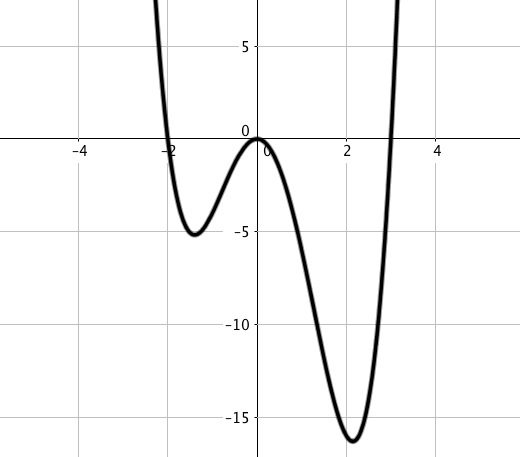
\includegraphics [width=0.3\textwidth ]{img-07-bloc2/sol-bloc2-polinomi1.png} 
\phantomsection
\item[\fontfamily{phv}\selectfont\color{blue}\textbf{\ref{exer:435}. }] \label{ans:435} 
\begin{tasks} \task $y=1$ asímptota horitzontal; $x=1$ i $x=3$ asímptotes verticals. La posició relativa és: $\limx {+\infty } f(x)=1$ per damunt; $\limx {-\infty } f(x)=1$ per davall. $\limx {1^-} f(x)=+\infty $, $\limx {1^+} f(x)=-\infty $, $\limx {3^-} f(x)=-\infty $, $\limx {3^+} f(x)=+\infty $. \task La funció té un mínim relatiu a $x=0$, $y=0$ i un màxim relatiu a $x=3/2$, $y=-3$ \task Gràfica: \par \includegraphics *[width=0.35\textwidth ]{img-07-bloc2/bloc2-10.png} \end{tasks}
\phantomsection
\item[\fontfamily{phv}\selectfont\color{blue}\textbf{\ref{exer:436}. }] \label{ans:436} 
L'única funció que presenta asímptota obliqua és c). L'asímptota obliqua és $y=2x+2$ i també té una asímptota vertical a $x=1$. La gràfica és la següent: \par \includegraphics *[width=0.4\textwidth ]{img-07-bloc2/bloc2-11.png} 
\phantomsection
\item[\fontfamily{phv}\selectfont\color{blue}\textbf{\ref{exer:437}. }] \label{ans:437} 
 $k=1/2$. La primera derivada $y'=(2x^2+2x+1)/(x+1/2)^2$ mai és zero. Sempre creix i per tant no té extrems.
\phantomsection
\item[\fontfamily{phv}\selectfont\color{blue}\textbf{\ref{exer:438}. }] \label{ans:438} 
$a=-6$ i $b=17$.
 \end{enumerate}

 \vspace{1cm} 
 
 \needspace{5\baselineskip} 
 \heading{Solucions del Tema 8}

\vspace{0.3cm}

 \needspace{3\baselineskip} 

\hyperlink{page.114}{\textbf{\em Pàgina 114}}
\begin{enumerate}
\phantomsection
\item[\fontfamily{phv}\selectfont\color{blue}\textbf{\ref{exer:491}. }] \label{ans:491} 
$(3/5, -4/5)$ i $(4/5, 3/5)$.
 \end{enumerate}
\vspace{0.3cm}

 \needspace{3\baselineskip} 

\hyperlink{page.115}{\textbf{\em Pàgina 115}}
\begin{enumerate}


 \needspace{2\baselineskip} 

\phantomsection
 \item[\fontfamily{phv}\selectfont\color{blue}\textbf{\ref{exer:494}. }] \label{ans:494}
 \begin{tasks}[column-sep=1em, item-indent=1.3333em](2)
	 \task $105.07^\circ $
	 \task $180^\circ $
\end{tasks}
 \end{enumerate}
\begin{enumerate}
\phantomsection
\item[\fontfamily{phv}\selectfont\color{blue}\textbf{\ref{exer:495}. }] \label{ans:495} 
$x=-1$, $\alpha =57.53^\circ $
 \end{enumerate}
\vspace{0.3cm}

 \needspace{3\baselineskip} 

\hyperlink{page.117}{\textbf{\em Pàgina 117}}
\begin{enumerate}
\phantomsection
\item[\fontfamily{phv}\selectfont\color{blue}\textbf{\ref{exer:521}. }] \label{ans:521} 
a) Punt final $(-3,2)$. b) Vector suma $\vvec +\vec w=(-2,3)$.
 \end{enumerate}
\begin{enumerate}


 \needspace{2\baselineskip} 

\phantomsection
 \item[\fontfamily{phv}\selectfont\color{blue}\textbf{\ref{exer:522}. }] \label{ans:522}
 \begin{tasks}[column-sep=1em, item-indent=1.3333em](2)
	 \task $-3$
	 \task $-11$
\end{tasks}
\phantomsection
\item[\fontfamily{phv}\selectfont\color{blue}\textbf{\ref{exer:523}. }] \label{ans:523} 
 a) $2\sqrt {3}$. b) Els dos tenen mòdul 2. c) angle $30^\circ $
\phantomsection
\item[\fontfamily{phv}\selectfont\color{blue}\textbf{\ref{exer:524}. }] \label{ans:524} 
a) $k=-2$. b) $k=\pm 4$. c) $k=-\sqrt {3}$
\phantomsection
\item[\fontfamily{phv}\selectfont\color{blue}\textbf{\ref{exer:525}. }] \label{ans:525} 
$(3/5, 4/5)$ o $(-3/5, -4/5)$
 \end{enumerate}

 \vspace{1cm} 
 
 \needspace{5\baselineskip} 
 \heading{Solucions del Tema 9}

\vspace{0.3cm}

 \needspace{3\baselineskip} 

\hyperlink{page.125}{\textbf{\em Pàgina 125}}
\begin{enumerate}
\phantomsection
\item[\fontfamily{phv}\selectfont\color{blue}\textbf{\ref{exer:550}. }] \label{ans:550} 
El feix de rectes és $r:$ $y-2=m(x-1)$. Passa-la a forma general i aplica que $d(r,O)=1$.
 \end{enumerate}
\vspace{0.3cm}

 \needspace{3\baselineskip} 

\hyperlink{page.127}{\textbf{\em Pàgina 127}}
\begin{enumerate}
\phantomsection
\item[\fontfamily{phv}\selectfont\color{blue}\textbf{\ref{exer:567}. }] \label{ans:567} 
Escriu el feix de rectes com $y=1-m(x-3)$, troba els punts de tall amb els eixos i comprova que l'àrea és $A=\frac {1}{2}(1+3m)(3+\frac {1}{m})=6$. Resol l'equació i troba $m=1/3$.
 \end{enumerate}
\vspace{0.3cm}

 \needspace{3\baselineskip} 

\hyperlink{page.128}{\textbf{\em Pàgina 128}}
\begin{enumerate}
\phantomsection
\item[\fontfamily{phv}\selectfont\color{blue}\textbf{\ref{exer:570}. }] \label{ans:570} 
Troba el peu de la perpendicular de $r$ pel punt $A$: $B=(0,3)$, $C=(1,4)$ i $D=(2,3)$ 
 \end{enumerate}
\vspace{0.3cm}

 \needspace{3\baselineskip} 

\hyperlink{page.129}{\textbf{\em Pàgina 129}}
\begin{enumerate}
\phantomsection
\item[\fontfamily{phv}\selectfont\color{blue}\textbf{\ref{exer:581}. }] \label{ans:581} 
 a) $k=-7$, b) $k=-7$
 \end{enumerate}
\begin{enumerate}
\phantomsection
\item[\fontfamily{phv}\selectfont\color{blue}\textbf{\ref{exer:582}. }] \label{ans:582} 
Contínua $\frac {x-3}{5}=\frac {y-2}{1}$, general $x-5y+7=0$.
\phantomsection
\item[\fontfamily{phv}\selectfont\color{blue}\textbf{\ref{exer:583}. }] \label{ans:583} 
a) $(x,y)=(2,-3)+\lambda (2, 5)$, b) $2x+3y-6=0$.
\phantomsection
\item[\fontfamily{phv}\selectfont\color{blue}\textbf{\ref{exer:584}. }] \label{ans:584} 
Si $k=-9/5$ són paral·leles, en altre cas són secants.
\phantomsection
\item[\fontfamily{phv}\selectfont\color{blue}\textbf{\ref{exer:585}. }] \label{ans:585} 
$k=\pm \sqrt {3}$.
\phantomsection
\item[\fontfamily{phv}\selectfont\color{blue}\textbf{\ref{exer:586}. }] \label{ans:586} 
$x=-3$, $y=-5$ i $x=17/5$ i $y=39/5$
 \end{enumerate}

 \vspace{1cm} 
 
 \needspace{5\baselineskip} 
 \heading{Solucions del Tema 10}

\vspace{0.3cm}

 \needspace{3\baselineskip} 

\hyperlink{page.132}{\textbf{\em Pàgina 132}}
\begin{enumerate}
\phantomsection
\item[\fontfamily{phv}\selectfont\color{blue}\textbf{\ref{exer:587}. }] \label{ans:587} 
Radi $\sqrt {8}$, $(x+1)^2+(y-3)^2=8$
 \end{enumerate}
\begin{enumerate}
\phantomsection
\item[\fontfamily{phv}\selectfont\color{blue}\textbf{\ref{exer:588}. }] \label{ans:588} 
Centre $O(1,0)$, radi $R=1$
 \end{enumerate}
\vspace{0.3cm}

 \needspace{3\baselineskip} 

\hyperlink{page.133}{\textbf{\em Pàgina 133}}
\begin{enumerate}
\phantomsection
\item[\fontfamily{phv}\selectfont\color{blue}\textbf{\ref{exer:589}. }] \label{ans:589} 
Centre $O(-1,1)$, semi-eixos $a=3$, $b=2$, focus $F'(-1-\sqrt {5}, 1)$ i $F'(-1+\sqrt {5}, 1)$. Excentricitat $e=0.745$
 \end{enumerate}
\begin{enumerate}
\phantomsection
\item[\fontfamily{phv}\selectfont\color{blue}\textbf{\ref{exer:590}. }] \label{ans:590} 
$\frac {x^2}{9}+\frac {y^2}{5}=1$ $e=2/3$
\phantomsection
\item[\fontfamily{phv}\selectfont\color{blue}\textbf{\ref{exer:591}. }] \label{ans:591} 
$\frac {x^2}{100}+\frac {y^2}{96}=1$
 \end{enumerate}
\vspace{0.3cm}

 \needspace{3\baselineskip} 

\hyperlink{page.134}{\textbf{\em Pàgina 134}}
\begin{enumerate}
\phantomsection
\item[\fontfamily{phv}\selectfont\color{blue}\textbf{\ref{exer:592}. }] \label{ans:592} 
$O(1,0)$, $a=4$, $b=3$, $F'(-4,0)$ i $F(6,0)$, asímptotes $y=\pm 3(x-1)/4$, $e=5/4$.
 \end{enumerate}
\begin{enumerate}
\phantomsection
\item[\fontfamily{phv}\selectfont\color{blue}\textbf{\ref{exer:593}. }] \label{ans:593} 
$a=b=1/\sqrt {2}$, $2{x^2}-2(y-2)^2=1$, $e=\sqrt {2}$.
 \end{enumerate}
\vspace{0.3cm}

 \needspace{3\baselineskip} 

\hyperlink{page.135}{\textbf{\em Pàgina 135}}
\begin{enumerate}
\phantomsection
\item[\fontfamily{phv}\selectfont\color{blue}\textbf{\ref{exer:594}. }] \label{ans:594} 
$x=\frac {1}{12}y^2$
 \end{enumerate}
\begin{enumerate}
\phantomsection
\item[\fontfamily{phv}\selectfont\color{blue}\textbf{\ref{exer:595}. }] \label{ans:595} 
$V(3,0)$, $F(0, 1)$, $d: y=-1$
\phantomsection
\item[\fontfamily{phv}\selectfont\color{blue}\textbf{\ref{exer:596}. }] \label{ans:596} 
És una hipèrbola. $d=c-a=0.75 a$
 \end{enumerate}
\vspace{0.3cm}

 \needspace{3\baselineskip} 

\hyperlink{page.137}{\textbf{\em Pàgina 137}}
\begin{enumerate}
\phantomsection
\item[\fontfamily{phv}\selectfont\color{blue}\textbf{\ref{exer:598}. }] \label{ans:598} 
$x^2+y^2-2x-2y-23=0$ o $(x-1)^2+(y-1)^2=25$. Té centre $O(1,1)$ i radi $R=5$.
 \end{enumerate}
\begin{enumerate}
\phantomsection
\item[\fontfamily{phv}\selectfont\color{blue}\textbf{\ref{exer:599}. }] \label{ans:599} 
$\frac {(x+1)^2}{25}+\frac {(y-3)^2}{9}=1$. La semi-distància focal $c=4$, els focus són $F'(-5,3)$ i $F(3,3)$, i l'excentricitat $e=0.8$.
\phantomsection
\item[\fontfamily{phv}\selectfont\color{blue}\textbf{\ref{exer:600}. }] \label{ans:600} 
Semi-eixos: $a=2$, $b=\sqrt {2}$, les asímptotes $y=\pm \frac {\sqrt {2}}{2}x$, semi-distància focal: $c=\sqrt {6}$ i l'excentricitat $e=1.225$.
\phantomsection
\item[\fontfamily{phv}\selectfont\color{blue}\textbf{\ref{exer:601}. }] \label{ans:601} 
La distància focus-directriu és $p=1/6$, l'equació $y-2=3 (x-1)^2$, la directriu és la recta $y=23/12$ i la posició del focus $F(1, 25/12)$.
\phantomsection
\item[\fontfamily{phv}\selectfont\color{blue}\textbf{\ref{exer:602}. }] \label{ans:602} 
a) El·lipse de centre $(1,0)$ i semi-eixos $a=2$, $b=1$. b) Circumferència de centre $(1,2)$ i radi $2$. c) Paràbola vertical de vèrtex $(0,-2)$ i distància Focus-directriu $p=3/2$.
 \end{enumerate}

 \vspace{1cm} 

 \needspace{5\baselineskip} 
 \heading{Solucions del Bloc III}

\vspace{0.3cm}

 \needspace{3\baselineskip} 

\hyperlink{page.138}{\textbf{\em Pàgina 138}}
\begin{enumerate}
\phantomsection
\item[\fontfamily{phv}\selectfont\color{blue}\textbf{\ref{exer:603}. }] \label{ans:603} 
a) $|\vec u|=\sqrt {2}$ b) $-2\vec u + 3\vvec =(-5,-4)$ c) $2\vec u \cdot (\vec u + \vvec )=6$
 \end{enumerate}
\begin{enumerate}
\phantomsection
\item[\fontfamily{phv}\selectfont\color{blue}\textbf{\ref{exer:604}. }] \label{ans:604} 
 $a=-2$
\phantomsection
\item[\fontfamily{phv}\selectfont\color{blue}\textbf{\ref{exer:605}. }] \label{ans:605} 
a) $m=-1$, $n=3$ b) $116.57^\circ $
\phantomsection
\item[\fontfamily{phv}\selectfont\color{blue}\textbf{\ref{exer:606}. }] \label{ans:606} 
$(\frac {1}{2}, \frac {\sqrt {3}}{2})$
\phantomsection
\item[\fontfamily{phv}\selectfont\color{blue}\textbf{\ref{exer:607}. }] \label{ans:607} 
$y=-8$
\phantomsection
\item[\fontfamily{phv}\selectfont\color{blue}\textbf{\ref{exer:608}. }] \label{ans:608} 
Paramètriques $\left \{\begin {array}{l} x=0+1t \\ y=3+2t \end {array}\right .$. General $2x-y-3=0$.
\phantomsection
\item[\fontfamily{phv}\selectfont\color{blue}\textbf{\ref{exer:609}. }] \label{ans:609} 
a) $k=-2$. b) $k=-4$
\phantomsection
\item[\fontfamily{phv}\selectfont\color{blue}\textbf{\ref{exer:610}. }] \label{ans:610} 
$A'(2,2)$
 \end{enumerate}
\vspace{0.3cm}

 \needspace{3\baselineskip} 

\hyperlink{page.139}{\textbf{\em Pàgina 139}}
\begin{enumerate}
\phantomsection
\item[\fontfamily{phv}\selectfont\color{blue}\textbf{\ref{exer:611}. }] \label{ans:611} 
El punt d'intersecció és $I(5,11)$ i el pendent de la recta $m'=1/3$. La recta és $y-11=\frac {1}{3}(x-5)$.
 \end{enumerate}
\begin{enumerate}
\phantomsection
\item[\fontfamily{phv}\selectfont\color{blue}\textbf{\ref{exer:612}. }] \label{ans:612} 
$P(\pm 5, 0)$
\phantomsection
\item[\fontfamily{phv}\selectfont\color{blue}\textbf{\ref{exer:613}. }] \label{ans:613} 
$Area=5$
\phantomsection
\item[\fontfamily{phv}\selectfont\color{blue}\textbf{\ref{exer:614}. }] \label{ans:614} 
Mediatriu AC: $x-2y+1=0$, Mediatriu $AB$: $14x-4y+21=0$, Circumcentre $O(-19/12, -7/24)$
\phantomsection
\item[\fontfamily{phv}\selectfont\color{blue}\textbf{\ref{exer:615}. }] \label{ans:615} 
Centre $O(1,-3)$ i radi $R=2$.
\phantomsection
\item[\fontfamily{phv}\selectfont\color{blue}\textbf{\ref{exer:616}. }] \label{ans:616} 
$\frac {x^2}{100}+\frac {y^2}{36}=0$
\phantomsection
\item[\fontfamily{phv}\selectfont\color{blue}\textbf{\ref{exer:617}. }] \label{ans:617} 
 a) Paràbola vertical amb vèrtex $V(0,0)$, $p=3$, focus $F(0,3/2)$ i directriu la recta $y=-3/2$. \par b) Hipèrbola de centre $O(1,-1)$, semieixos $a=4$, $b=3$, semi-distància focal $c=5$. Excentricitat $e=1.25$. Focus a $F'(-4,-1)$, $F(6,-1)$. Asímptotes $y+1=\pm \frac {3}{4}(x-1)$. \par \begin {center} 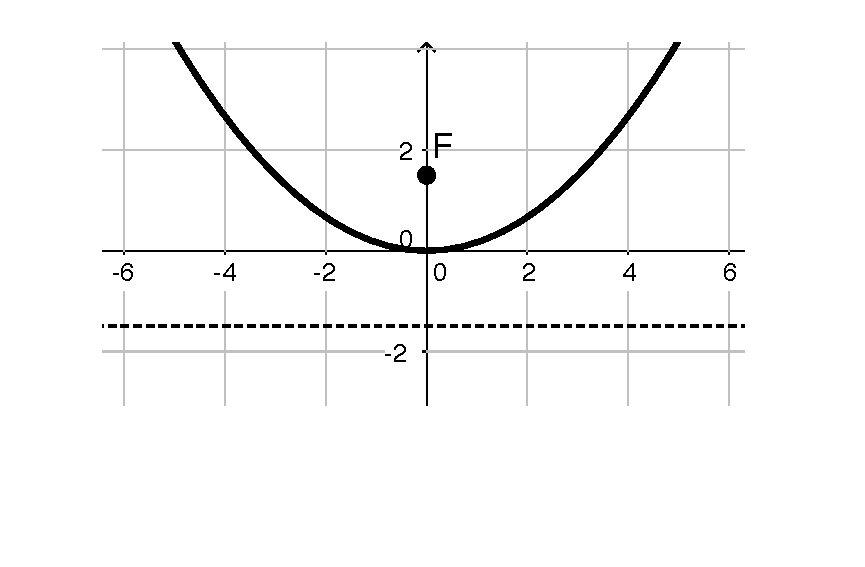
\includegraphics [height=3cm]{img-10-bloc3/bloc3-sol-14a} 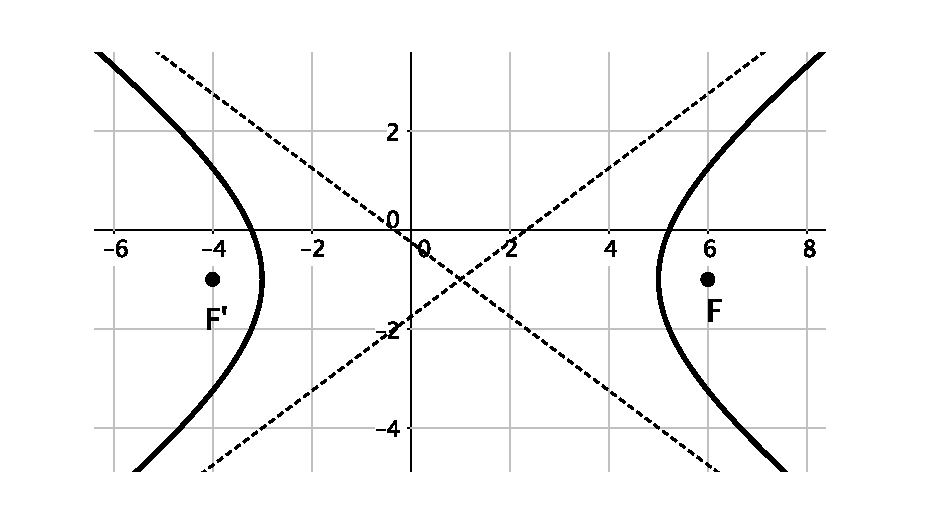
\includegraphics [height=3cm]{img-10-bloc3/bloc3-sol-14b} \end {center} 
\phantomsection
\item[\fontfamily{phv}\selectfont\color{blue}\textbf{\ref{exer:618}. }] \label{ans:618} 
$a=39.3$ ua, $c=9.8$ ua, $b=38.06$ ua. $\dfrac {x^2}{39.3^2}+\dfrac {y^2}{38.06^2}=1$
 \end{enumerate}

 \vspace{1cm} 
 
 \needspace{5\baselineskip} 
 \heading{Solucions del Tema 11}

\vspace{0.3cm}

 \needspace{3\baselineskip} 

\hyperlink{page.143}{\textbf{\em Pàgina 143}}
\begin{enumerate}
\phantomsection
\item[\fontfamily{phv}\selectfont\color{blue}\textbf{\ref{exer:620}. }] \label{ans:620} 
\begin {tabular}{c|c|c|c|c|c|c|c}\hline $x$ & 0 & 1 & 2 & 3 & 4 & 5 & 6 \\\hline $f$ & 2 &4 & 21 & 15 & 6 & 1 &1 \\ \end {tabular} \par c) $\bar x =2.52$ i $\sigma =0.496$ fills. 
 \end{enumerate}
\vspace{0.3cm}

 \needspace{3\baselineskip} 

\hyperlink{page.144}{\textbf{\em Pàgina 144}}
\begin{enumerate}
\phantomsection
\item[\fontfamily{phv}\selectfont\color{blue}\textbf{\ref{exer:621}. }] \label{ans:621} 
\begin {tabular}{c|c|c|c|c|c}\hline $x$ & 2.5-3 & 3-3.5 & 3.5-4 & 4-4.5 & 4.5-5\\\hline $f$ & 6 & 10 & 11 & 8 & 5 \\ \end {tabular} \par c) $\bar x =3.7$ i $\sigma =0.62$ kg. 
 \end{enumerate}
\vspace{0.3cm}

 \needspace{3\baselineskip} 

\hyperlink{page.148}{\textbf{\em Pàgina 148}}
\begin{enumerate}
\phantomsection
\item[\fontfamily{phv}\selectfont\color{blue}\textbf{\ref{exer:627}. }] \label{ans:627} 
$y=1.194+4.78(x-0.232)$, el pendent és la constant elàstica $k=4.78$ N/m. L'allargament per a $y=2$ N és $x=40$ cm. És bastant fiable ja que $r=0,998$.
 \end{enumerate}
\vspace{0.3cm}

 \needspace{3\baselineskip} 

\hyperlink{page.149}{\textbf{\em Pàgina 149}}
\begin{enumerate}
\phantomsection
\item[\fontfamily{phv}\selectfont\color{blue}\textbf{\ref{exer:629}. }] \label{ans:629} 
a) $r=-0.997$ correlació negativa forta; \quad b) Recta de regressió $y=-0.2632 x+10.37$, altura $y=8.84$ m. \quad c) $x=66$ hores
 \end{enumerate}
\vspace{0.3cm}

 \needspace{3\baselineskip} 

\hyperlink{page.152}{\textbf{\em Pàgina 152}}
\begin{enumerate}
\phantomsection
\item[\fontfamily{phv}\selectfont\color{blue}\textbf{\ref{exer:643}. }] \label{ans:643} 
a) Hi ha una correlació lineal positiva forta $\sigma _{xy}=1.71$ i $r=0.91$\par b) $y=0.87x+2.25$. Es cometen 4.86 errors.
 \end{enumerate}
\begin{enumerate}
\phantomsection
\item[\fontfamily{phv}\selectfont\color{blue}\textbf{\ref{exer:644}. }] \label{ans:644} 
Hi ha una correlació positiva molt feble. $\sigma _{xy}=6.8$, $r=0.60$, $y=4x-95.3$
\phantomsection
\item[\fontfamily{phv}\selectfont\color{blue}\textbf{\ref{exer:645}. }] \label{ans:645} 
a) $y=0.1x+6.65$\quad b) No seria gens fiable fer prediccions en aquest cas ja que $r=0.16$ és molt inferior a 1.
 \end{enumerate}
\end{multicols}

\end{document} 
